\documentclass{article}
\usepackage[utf8]{inputenc}

\usepackage{amsthm}
\usepackage{amsmath}
\usepackage{amssymb}

% BIBLIOGRAPHY STUFF

\usepackage[all]{xy} % For diagrams
\usepackage[symbol]{footmisc} % For symbol footnote

\usepackage{xargs}                      % Use more than one optional parameter in a new commands
\usepackage[pdftex,dvipsnames]{xcolor}  % Coloured text etc.
% 
\usepackage[colorinlistoftodos,prependcaption,textsize=tiny]{todonotes}

% TODO STUFF
\newcommandx{\needtodo}[2][1=]{\todo[linecolor=red,backgroundcolor=red!25,bordercolor=red,#1]{#2}}
\newcommandx{\change}[2][1=]{\todo[linecolor=blue,backgroundcolor=blue!25,bordercolor=blue,#1]{#2}}
\newcommandx{\info}[2][1=]{\todo[linecolor=OliveGreen,backgroundcolor=OliveGreen!25,bordercolor=OliveGreen,#1]{#2}}
\newcommandx{\improvement}[2][1=]{\todo[linecolor=Plum,backgroundcolor=Plum!25,bordercolor=Plum,#1]{#2}}
\newcommandx{\thiswillnotshow}[2][1=]{\todo[disable,#1]{#2}}

% Tikz stuff
\usepackage{tikz}
\usetikzlibrary{patterns}
\usepackage{hyperref}
\usepackage[linesnumbered,lined,commentsnumbered]{algorithm2e} % For writing beautiful algoritms

%\theoremstyle{plain}
%\newtheorem{thm}{Theorem}[chapter] % reset theorem numbering for each chapter

%\theoremstyle{definition}
%\newtheorem{defn}[thm]{Definition} % definition numbers are dependent on theorem numbers
%\newtheorem{exmp}[thm]{Example} % same for example numbers

% Custom commands and stuff
\theoremstyle{plain}
\newtheorem{theorem}{Theorem}[section]

\theoremstyle{definition}
\newtheorem{proposition}[theorem]{Proposition}
\newtheorem{lemma}[theorem]{Lemma}
\newtheorem{definition}[theorem]{Definition}

% Custon commands to make mathmode-ideals and stuff more easy my man
% \mathfrak stuff
\newcommand{\frakp}{\mathfrak{p}}
\newcommand{\fraka}{\mathfrak{a}}
\newcommand{\frakb}{\mathfrak{b}}
\newcommand{\frakI}{\mathfrak{I}}
\newcommand{\frakF}{\mathfrak{F}}
\newcommand{\frakP}{\mathfrak{P}}
\newcommand{\frakq}{\mathfrak{q}}
\newcommand{\calI}{\mathcal{I}}
\newcommand{\calJ}{\mathcal{J}}
% Class group
\newcommand{\CL}{\text{CL}}
% mathcal
\newcommand{\OO}{\mathcal{O}}
% Complex conjugate
\newcommand{\compconj}[1]{%
  \overline{#1}%
}
\let\vec\boldsymbol % change how \vec works
\newcommand{\suchthat}{\;|\;}
\newcommand{\modulo}{\mathop{}\!\mathrm{\; mod \;}}

% Mathbb-s
\newcommand{\ZZ}{\mathbb{Z}}
\newcommand{\QQ}{\mathbb{Q}}
\newcommand{\RR}{\mathbb{R}}
\newcommand{\CC}{\mathbb{C}}
\newcommand{\Norm}{\mathrm{N}}
\newcommand{\Trace}{\mathrm{Tr}}
\newcommand{\inverse}{^{-1}}

\title{Master Thesis}
\author{Thor Tunge}
\date{Datum}


\begin{document}

\maketitle

\newpage

\section*{Abstract}
We study the security of lattice based crypto system based on ideal lattices and principal ideal lattices. for the latter, there exists a quantum polynomial attack. For systems which use ideal lattices and has a basis for the lattice as public key, we show that they are somewhat insecure.

\newpage
\tableofcontents

\newpage
\section{Introduction}
    \label{Section:Introduction}\needtodo{Talk about FHE?}
    With the advent of quantum computers cryptographic schemes based on problems not easily broken by quantum algorithms have risen in popularity. A group of such problems arise in the theory of lattices (Section \ref{Section:Lattice Theory}. A lattice is a discrete subspace of \(\mathbb{R}^n\). Some central, hard problems that naturally arise in lattice-based cryptography is to find the shortest vector in the lattice, the \emph{Shortest Vector Problem} (SVP), and finding the closest lattice-point to a vector in \(\mathbb{R}^n\), the \emph{Closest Vector Problem}. These two problems are closely related.\\
    % Input a figure of some lattice stuff
    \begin{figure}[h]
\center
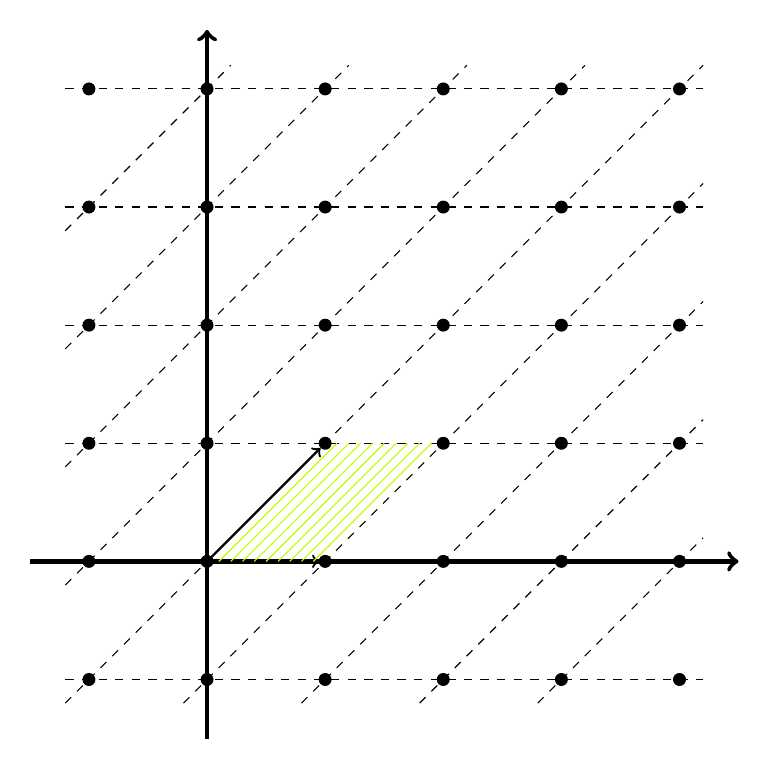
\begin{tikzpicture}[scale=1.5]

% AXES
\draw [ultra thick, ->] (-1.5, 0) -- (4.5, 0);
\draw [ultra thick, ->] (0, -1.5) -- (0, 4.5);

% BASIS VECTORS
\draw [thick, ->] (0, 0) -- (0.95, 0);
\draw [thick, ->] (0, 0) -- (0.96, 0.96);

% HORIZONTAL LINES
\draw [dashed, thin] (-1.2, 4) -- (4.2, 4);
\draw [dashed, thin] (-1.2, 3) -- (4.2, 3);
\draw [dashed, thin] (-1.2, 2) -- (4.2, 2);
\draw [dashed, thin] (-1.2, 1) -- (4.2, 1);
\draw [dashed, thin] (-1.2, -1) -- (4.2, -1);

% SKEW LINES
\draw [dashed] (-1.2, -0.2) -- (3.2, 4.2);
\draw [dashed] (-1.2, 0.8) -- (2.2, 4.2);
\draw [dashed] (-1.2, 1.8) -- (1.2, 4.2);
\draw [dashed] (-1.2, 2.8) -- (0.2, 4.2);
\draw [dashed] (-1.2, -1.2) -- (4.2, 4.2);
\draw [dashed] (-0.2, -1.2) -- (4.2, 3.2);
\draw [dashed] (0.8, -1.2) -- (4.2, 2.2);
\draw [dashed] (1.8, -1.2) -- (4.2, 1.2);
\draw [dashed] (2.8, -1.2) -- (4.2, 0.2);

% All intersection points
\draw[fill] (1,1) circle [radius=0.025];\draw[fill](-1,-1)circle [radius=0.050];\draw[fill](-1,0)circle [radius=0.050];\draw[fill](0,-1)circle [radius=0.050];\draw[fill](0,0)circle [radius=0.050];\draw[fill](1,-1)circle [radius=0.050];\draw[fill](1,0)circle [radius=0.050];\draw[fill](2,-1)circle [radius=0.050];\draw[fill](2,0)circle [radius=0.050];\draw[fill](3,-1)circle [radius=0.050];\draw[fill](3,0)circle [radius=0.050];\draw[fill](4,-1)circle [radius=0.050];\draw[fill](4,0)circle [radius=0.050];\draw[fill](-1,1)circle [radius=0.050];\draw[fill](-1,2)circle [radius=0.050];\draw[fill](0,1)circle [radius=0.050];\draw[fill](0,2)circle [radius=0.050];\draw[fill](1,1)circle [radius=0.050];\draw[fill](1,2)circle [radius=0.050];\draw[fill](2,1)circle [radius=0.050];\draw[fill](2,2)circle [radius=0.050];\draw[fill](3,1)circle [radius=0.050];\draw[fill](3,2)circle [radius=0.050];\draw[fill](4,1)circle [radius=0.050];\draw[fill](4,2)circle [radius=0.050];\draw[fill](-1,3)circle [radius=0.050];\draw[fill](-1,4)circle [radius=0.050];\draw[fill](0,3)circle [radius=0.050];\draw[fill](0,4)circle [radius=0.050];\draw[fill](1,3)circle [radius=0.050];\draw[fill](1,4)circle [radius=0.050];\draw[fill](2,3)circle [radius=0.050];\draw[fill](2,4)circle [radius=0.050];\draw[fill](3,3)circle [radius=0.050];\draw[fill](3,4)circle [radius=0.050];\draw[fill](4,3)circle [radius=0.050];\draw[fill](4,4)circle [radius=0.050];

% Fundamental paraleliped (?)

\draw[thin,color=lime] (0.1,0) -- (1.1, 1);
\draw[thin,color=lime] (0.2,0) -- (1.2, 1);
\draw[thin,color=lime] (0.3,0) -- (1.3, 1);
\draw[thin,color=lime] (0.4,0) -- (1.4, 1);
\draw[thin,color=lime] (0.5,0) -- (1.5, 1);
\draw[thin,color=lime] (0.6,0) -- (1.6, 1);
\draw[thin,color=lime] (0.7,0) -- (1.7, 1);
\draw[thin,color=lime] (0.8,0) -- (1.8, 1);
\draw[thin,color=lime] (0.9,0) -- (1.9, 1);



\end{tikzpicture}
\caption{Lattice with basis \(\mathfrak{B} = \{(1, 0), (1, 1)\}\). This lattice is isomorphic to the lattice with basis vectors \((1, 0)\) and \((-1, 1)\).}
\label{Figure:Lattice1}
\end{figure}
    
    Many efficient cryptosystems rely on \emph{ideal lattices}, which correspond to ideals in a certain ring\footnote{Namely \(\mathbb{Z}[X]/\langle f(x)\rangle\) for an irreducible \(f(x)\)}. Solving SVP in such lattices boils down to finding a 'short' generator for the ideal. We often assume that there exists a short generator, so that the search can succeed. There are two steps in finding such a generator for a principal ideal \cite{Recover Short Gen}.
    
    Firstly, find a generator for a principal ideal, which need not be short. This is called the \emph{principal ideal problem}. The results of \cite{Find Generator Classic} has show that this is possible to do classically in sub-exponential time, namely \(2^{N^{1/2 + O(1)}}\). Additionally, there exists a quanum polynomial time algorithm from \cite{Find Generator Quantum} which finds such a generator. Secondly, after a generator is found, transform it into a 'short' generator and thereby recover the secret key of the cryptosystems. A proof of the second part of the process was provided by \cite{Recover Short Gen}.
    
    The security of many modern lattice based cryptography schemes is based on the hardness of these problems. In particular, the security of the fully homomorphic scheme by Gentry \cite{Gentry} and schemes based on his methods, such as the one by Smart and Vercauteren\needtodo{Find source for this}, hinges on solving the SG-PIP problem. There is a classical reduction from SG-PIP to (LWE) by Peikert.\cite{Reduction PG-PIP LWE}\improvement{Read this source}. So finding a good solution to SG-PIP means that LWE is not hard, and assuming LWE is hard then these cryptosystems are secure in some sense.\improvement{Elaborate}\par
    
    The structure of this thesis is as follows: We start by introducing the general algebraic number theory required to understand the machinery used in various algorithms and problems. Then we present basic lattice theory and the hard problems used in cryptography associated with lattices. We discuss the relationship between hard problems and how they relate to security. Next, we present the algorithms for the first part of SG-PIP, discussing both the sub-exponential classic and quantum polynomial algorithm. From there we show how a found generator can be made 'short'. Any specific theory needed in either of these algorithms will be presented in that chapter.\newpage
\subsection{Glossary}
    To keep consistent notation, use the following notation my man
    \begin{itemize}
        \item \(K, L\) are a number fields, \(L\) extension of \(K\).
        
        \item \(R = \OO_K\): Ring of integers. Omit \(K\) if it is clear.
        
        \item \(\alpha\) are integral elements
        
        \item \(\Lambda\) is a lattice
        
        \item \(\mathcal{B}\) and \(\mathcal{B}^\vee\) are the basis and dual basis, respectively.
        
        \item \(\vec{b}\) and \(\vec{b}^\vee\) are basis vectors and dual basis vectors, respectively
        
        \item \(\fraka, \frakb\) are ideals
        
        \item \(\frakp, \frakq\) are prime ideals
        
        \item \(\calI\) is the group of fractional ideals, or just set of ideals
        
        \item Keep \(U\) to mean group of units of something, probably group of roots of unity.
        
        \item \(\sigma\) is the cannonical embedding. \(\tau\) is the coordiante embedding?
        
        \item \(d\) is a divisor.
        
    \end{itemize}
\newpage
\section{Preliminaries}
\label{Section:Preliminaries}
Let \(a = (a_1,\dots ,a_n) \in\mathbb{R}^n\) be a vector, then denote by
\begin{align*}
    ||a||_l = \left(\sum\limits_{i = 1}^l |a_i|^n\right)^\frac{1}{l}
\end{align*}
the \(l\)-norm. We will almost always use the 2-norm because it is the best norm.\par
We use the notation \(\lceil a\rfloor\) to denote the closest integer to \(a\).\par
For problems \(A\) and \(B\), the notation \(A\leq B\) will be used to indicate that \(A\) is at least as hard as \(B\). In other words \(A\leq B\implies A \text{ reduces to }B\). Two equivalent problems are denoted \(A=B\). \par
We talk a lot about rings of integers. Here it is helpful to think about certain elements as denominators. Throughout this thesis we will denote these elements by \(d\) and keep the notation consistent throughout.

\newpage
\section{Algebraic Number Theory}
\label{Section:Algebraic Number Theory}
    Algebraic number theory is the study of finite extensions \(K\) of \(\QQ\). We generalize the notion of integers, study the ideals in this 'new' ring of integers and extend the notion of ideal to give the set of ideals a group structure. Some of the notion here makes sense more more general extensions, but we state them only in the spirit of finite extensions of \(\QQ\). Throughout this section (and the thesis in general), \(K\) denotes a finite extension of \(\QQ\).
\subsection{Norm and Trace}
    To get some geometry on certain algebraic structures, we want to define the norm and trace of elements. 
    \begin{definition}[Norm and Trace]
    Let \(K/\QQ\) be a finite field extension. Consider the multiplication map
    \begin{align*}
        \begin{split}
            \mu_\alpha: & K\rightarrow K\\
            &x\mapsto\alpha x.
        \end{split}
    \end{align*}
    By fixing a \(\QQ\)-basis of \(K\), we can define the \emph{determinant} and \emph{trace} maps to be
    \begin{align*}
        \begin{split}
            \emph{N}_{K/\QQ}(\alpha) & = \emph{det}(\mu_\alpha)\\
            \emph{Tr}_{K/\QQ}(\alpha) & = \emph{Tr}(\mu_\alpha)
        \end{split}
    \end{align*}
    \end{definition}
    Notice that both maps map \(K\rightarrow \QQ\)\improvement{why is this?}, and that the determinant map is multiplicative while the trace map is additive. It also makes sense to fix a \(\QQ\) basis since the extension is finite. A property we will often use is that the norm and trace for integers are both rational integers. We state it here without proof.
    \begin{proposition}[\cite{Basic Algebraic Number Theory}]
        The norm and trace of \(\alpha\in \OO\) are rational integers. 
    \end{proposition}
    Additionally, \(N(\alpha) = \pm 1 \Leftrightarrow \alpha\in\OO^*\): The norm of an element is \(\pm1\) if, and only if, it is a unit in the ring of integers.\par
    \cite{First R-LWE}A number field \(K = \QQ(\zeta)\) has \(n\) exactly ring embeddings \(\sigma_i : K\rightarrow \mathbb{C}\), by sending \(\zeta\) to a root of the minimal polynomial \(f(X)\) of \(\zeta\). Since the complex roots come in conjugate pairs, so does the embeddings. Denote by \(s_1\) the number of real embeddings and by \(s_2\) the number of \emph{pairs} or complex embeddings. As such, \(n = s_1 + 2s_2\). By convention, order the embeddings as follows: \(\sigma_1, \dots \sigma_{s_1}\) are the real embeddings. The complex ones is ordered such that \(\sigma_{s_1 + s_2 + j} = \compconj{\sigma_{s_1 + j}}\) for \(j\in\{1,\dots ,s_2\}\). Therefore, with increasing \(j\) we have first the \(s_1\) real embeddings, then the \(s_2\) complex embeddings \emph{with no conjugates among themselves} and lastly the \(s_2\) conjugates. Now we define
    \begin{align*}
        \sigma(x) = (\sigma_1(x), \dots , \sigma_{n}(x))
    \end{align*}
     as the \emph{canonical} embedding of \(K\mapsto \RR^{s_1}\times \mathbb{C}^{2s_2}\)\improvement{is this defined elsewhere?}. Notice that this means that certain elements of \(K\) will have slightliy unusual norms. Take \(K = \QQ(\zeta_p)\) a cyclotomic field. A root of unity, which 'usually' has norm 1, \(\zeta_p\) will be embedded as
     \begin{align*}
         \sigma(\zeta_p) = (\zeta_p, \zeta_p^2, \dots , \zeta_p^{n-1})
     \end{align*}
     which means that its norm \(||\zeta_p|| := ||(\zeta_p, \dots ,\zeta_p^{n-1}||_2 = \sqrt{n}\).
\subsection{Ring of Integers}
    A lot of the background for solving the lattice problems lie in algebraic number theory. Here, we generalize number theory over the field \(\QQ\) and its ring of integers \(\ZZ\) to an extension field \(K\supseteq\QQ\) and \emph{its} ring of integers, denoted \(\OO_K\). As to not cause confusion, we call \(\ZZ\) the \emph{rational integers}. We call an extension field \(K\) of \(\QQ\) a \emph{number field}. To have a discussion of a generalized ring of integers, we need to define it:
    \begin{definition}[Integral Element and Set of Algebraic Integers]
        Let \(K\) be a field. We say that \(n\) is an \emph{integral element} in \(K\) if \(n\) is a root of a monic polynomial with rational integer coefficients. The \emph{set of algebraic integers} of \(K\), denoted \(\OO_K\) is the set of all integral elements of \(K\). 
    \end{definition}
    Trivially, a rational integer \(n\) is the root of \(x - n\) and therefore we have \(\ZZ\subseteq\OO_K\). We want to prove that \(\OO_K\) is a ring, and to do that we need to following proposition:
    \begin{proposition}
    \label{Prop: Equivalence Algebraic Integer Integer Minimal Polynomial}
        The minimal polynomial of \(\alpha\in K\) has integer coefficients if, and only if, \(\alpha\) is an algebraic integer.
    \end{proposition}
    \begin{proof}
        Assume that the minimal polynomial of \(\alpha\), say \(g(X)\) has integer coefficients. Since \(g(\alpha) = 0\) by the definition of minimal polynomial, \(\alpha\) is an algebraic integer. \par
        Assume now that \(\alpha\) is an algebraic integer. By definition, there exists an \(f(X)\in\ZZ [X]\) such that \(f(\alpha) = 0\). If \(f(X)\) is the minimal polynomial we are done. Let therefore \(g(X)\) be the minimal polynomial of \(\alpha\). We need to show that \(g(X)\) also has integer coefficients. Since \(g(X)\) is the minimal polynomial, we have that 
        \begin{align*}
            f(X) = g(X)h(X)
        \end{align*}
        for some \(h(X)\). Now assume, towards a contradiction, that \(g(X)\) has rational coefficients, i.e. that at least one denominator is divisible by a prime \(p\). If \(g(X)\) has a rational coefficient, then one of them must be divisible by \(p\) (by fundamental theorem of algebra). Let \(u\) be the smallest integer such that \(p^ug(X)\) has no denominators divisible by \(p\). Similarly, let \(v\) be the smallest integer such that \(p^vh(X)\) has no denominators divisible by \(p\). Now, since the left side of
        \begin{equation}
        \label{Eq: Minimal Polynomial}
           p^ug(X)p^vh(X) = p^{u + v}f(X)
        \end{equation}
        has no denominators divisible by \(p\). If we now regard Equation \eqref{Eq: Minimal Polynomial} as an equation in \(\mathbb{F}_p[X]\), since \(f(X)\) has integer coefficients, the right side is \(0\). Since we have removed all \(p=0\in\mathbb{F}_p\) from the left side, regarding it as polynomials in \(\mathbb{F}_p\) makes sense. Therefore,
        \begin{align*}
            p^ug(X)p^vh(X) = 0\in\mathbb{F}_p[X],
        \end{align*}
        and because we chose \(u\) and \(v\) to be minimal, neither \(p^ug(X)\) nor \(p^vh(X)\) are zero-polynomials. Since \(\mathbb{F}_p[X]\) has no zero divisors, this leads to a contradiction and we conclude that \(g(X)\in\ZZ[X]\).
    \end{proof}
    Towards a goal of proving that \(\OO_K\) is a ring, we also use a relationship between an algebraic integer \(\alpha\) and \(\ZZ[\alpha]\).
    \begin{proposition}
    \label{Prop: Equivalence Algebraic Integer and Finitely Generated Z-module}
        Let \(\alpha\in K\). Then \(\alpha\) is an algebraic integer if, and only if, \(\ZZ[\alpha]\) is finitely generated as a \(\ZZ\)-module. 
    \end{proposition}
    \begin{proof}
        Assume \(\alpha\) is an algebraic integer, and let \(g(X)\) be its minimal polynomial of degree \(m\). By \ref{Prop: Equivalence Algebraic Integer Integer Minimal Polynomial} we have that \(g(X)\) is monic with integer coefficients and can therefore write
        \begin{align*}
            g(X) = X^m + \hat{g}(X)
        \end{align*}
        for some \(\hat{g}(X)\). Because \(g(\alpha) = 0\) we can write \(\alpha^m = -\hat{g}(\alpha)\) where \(\text{deg}\;\hat{g}(X) < \text{deg}\;g(X)\). This means that any \(\alpha^u\) can be written as a \(\ZZ\)-linear combination of \(\{1, \alpha, \alpha^2,\dots ,\alpha^{m-1}\}\) which generate \(\ZZ[\alpha]\).\par
        Now assume that \(\ZZ[X]\) is finitely generated with generators \(\{a_0, a_1,\dots ,a_{m - 1}\}\). Let \(f_i(X), i=0,\dots m-1\) be such that \(a_i = f(\alpha)\) for an \(\alpha\in K\). Now pick an \(N>\text{deg}\;f_i\) for all \(i=0,\dots ,m-1\). Since
        \begin{align*}
            \alpha^N = \sum\limits_{i= 0}^{m-1}a_ib_i\quad\text{for some }b_i\in\ZZ,
        \end{align*}
        choose
        \begin{align*}
            f(X) = X^N - \sum\limits_{i = 1}^{m - 1}f_i(X)b_i.
        \end{align*}
        Because we chose \(N\) to be larger than all \(\text{deg}\;f_i(X)\), \(f(X)\) is monic and has integer coefficients. Furthermore, \(f(\alpha) = 0\) so \(\alpha\) is an algebraic integer.
        \end{proof}
        \begin{theorem}
        \(\OO_K\) is a ring.
        \end{theorem}
        \begin{proof}
        Let \(\alpha, \beta \in \OO_K\). By Proposition \ref{Prop: Equivalence Algebraic Integer and Finitely Generated Z-module} we have that \(\ZZ[\alpha]\) and \(\ZZ[\beta]\) are finitely generated, and therefore \(\ZZ[\alpha, \beta]\) is finitely generated. Regarding \(\ZZ[\alpha, \beta]\) as a ring, we have that \(\alpha\beta, \alpha\pm\beta\in\ZZ[\alpha, \beta]\). Now, since \(\ZZ[\alpha\beta]\) and \(\ZZ[\alpha\pm\beta]\) are both subrings of \(\ZZ[\alpha, \beta]\), they are finitely generated. By Proposition \ref{Prop: Equivalence Algebraic Integer and Finitely Generated Z-module} again, we conclude that \(\alpha\beta\) and \(\alpha\pm\beta\) are algebraic integers and \(\OO_K\) is therefore a ring. 
    \end{proof}
    If we let the field be \(\QQ\), then the ring of integers equals the rational integers \(\ZZ = \OO_\QQ\). To see this, recall Gauss' \needtodo{Check this is the right lemma} lemma that every root of a monic polynomial with rational coefficients is a rational integer. As \(\ZZ\subseteq\OO_K\) this is the simplest form the ring of integers can have. \(\OO_K\) might be more complicated than this. Without restrictions of the field \(K\), the ring of integers can be quite hard to determine. But alas, we can find some structure:
    \begin{proposition}
    \label{Prop: QO equals K}
        Let \(K\) be a number field with ring of integers \(\OO_K\). Then \(\QQ\OO_K = K\).
    \end{proposition}
    \begin{proof}
        Clearly \(\QQ\OO_K\subseteq K\).\par
        \underline{\(K\subseteq\QQ\OO_K\)}: Now assume \(\alpha\in K\). Let \(f(X)\) be the minimal polynomial of \(\alpha\). Let \(d\) be the least common multiple of the coefficients of \(f(X)\). Then let 
        \begin{align*}
            d^{\text{deg}\;f(X)}f(\frac{X}{d}) = g(X).
        \end{align*}
        By design, \(df(X)\) will have only integer coefficients, and \(d^{\text{deg}\;f(X)}f(X/d)\) will be monic. Additionally, \(g(\alpha d) = f(\alpha) = 0\), so \(g(X)\) is a monic polynomial with integer coefficients that has \(\alpha d\) as a root. By Proposition \ref{Prop: Equivalence Algebraic Integer and Finitely Generated Z-module} we get that \(\alpha d\in\OO_K\subseteq\QQ\OO_K\) which we wanted to prove. 
    \end{proof}
    From this proof we get a small lemma:
    \begin{lemma}
        \label{Lemma: a in K can be ad in O}
        For any \(\alpha\in K\), there exists \(d\in\ZZ\) such that \(\alpha d \in\OO\).
    \end{lemma}
    \begin{proof}
        See proof of Proposition \ref{Prop: QO equals K}.
    \end{proof}
    Notice that the \(d\in\ZZ\) acts as a denominator, multiplying \(\alpha\) by \(d\) cancels whatever a denominator means for an element in \(K\) and gives us an integral element. \par
    Now we have the tools to prove a central part of the ring of integers.
    \begin{theorem}
    \label{Thm: O is free}
        The ring of integers \(\OO_K\) is a free abelian group of rank \(n = [K:\QQ]\)
    \end{theorem}
    \begin{proof}
        From Lemma \ref{Lemma: a in K can be ad in O} we know that there exists a \(\QQ\)-basis \(\{\alpha_1,\dots ,\alpha_n\}\) of \(K\) with \(\alpha_i\in\OO_K\) for all \(i = 1,\dots n\). We can therefore write
        \begin{align*}
            x = \sum\limits_{i = 1}^{n} c_i\alpha_i
        \end{align*}
        \needtodo{Finish this proof}\cite{Basic Algebraic Number Theory}
    \end{proof}
    
\subsection{Ideals of Ring of Integers}
    We now know what \(\OO_K\) is a ring and finitely generated as a \(\ZZ\)-module. An important part of the ring of integers is its ideals. We define the ideal norm as
    \begin{definition}[Ideal Norm]
    The norm of an ideal \(\fraka\subseteq \OO_K\) is
    \begin{align*}
        N(\fraka) = |\OO_K/\fraka|
    \end{align*}
    \end{definition}
    It can be shown that the norm of an ideal if finite. Indeed, we will show later that both \(\OO\) and any ideal \(\fraka\subseteq\OO\) have a basis with the same number of elements. We see that a 'large' ideal in the subset sense will have a small norm. This means that maximal ideals are ideals with small norm.\par
    
    For primes in \(\ZZ\) we have two equivalent definitions: A number is prime if \(p=ab\implies a\text{ or }b \) is a unit \textit{or} \(p|ab\implies p|a \text{ or }p|b\). However, this definition does not generalize. \cite{Basic Algebraic Number Theory}. In the general case, we differentiate between these two properties, and call the first one \emph{irreducible} and the second one \emph{prime}. We can therefore define a prime ideal as follows:
    \begin{definition}[Prime Ideal]
        An ideal \(\mathfrak{p}\) is \emph{prime} if for any ideals \(\mathfrak{a}\) and \(\mathfrak{b}\)
        \begin{align*}
            \mathfrak{a}\mathfrak{b}\subseteq \mathfrak{p} \implies \mathfrak{a}\subseteq \mathfrak{p}\quad\text{or}\quad \mathfrak{b}\subseteq \mathfrak{p}
        \end{align*}
    \end{definition}
    
    A special property of prime ideals in \(\OO\) is that they are all maximal.
    \begin{proposition}
        \label{Prop: Every Prime Ideal in O is Maximal}
        Every prime ideal in \(\OO\) is maximal.
    \end{proposition}
    \begin{proof}
        Any ideal \(I\subseteq \OO\) is maximal if, and only if, the quotient \(\OO/I\) is a field. We therefore show that this is the case for \(\frakp\). Take \(x\in\OO/\frakp\). Because \(\frakp\) is prime, \(\OO/\frakp\) is an integral domain. Therefore, the kernel of the multiplication map \(\mu_x:\OO/\frakp \rightarrow \OO/\frakp\) is 0 and thus \(\mu_x\) is injective. Since \(\OO/\frakp\) is finite\needtodo{has not been shown}, \(\mu_x\) is also surjective so it is a bijection. Take \(x\inverse = \mu_x\inverse(1)\). Now \(xx\inverse = x\mu_x\inverse(1) = 1 \). We showed that every element of \(\OO/\frakp\) has an inverse, thus it is a field and conclude that \(\frakp\) is maximal.
    \end{proof}
    We eventually want to prove that any ideal is the unique product of prime ideals up to order of the factors. Towards this goal we show the following inclusion.
    \begin{proposition}
    \label{Prop: Prime Subset of Ideal}
    Let \(I\) be a non-zero ideal of \(\OO\). Then there exists prime ideals \(\frakp_1,\dots\frakp_r\) of \(\OO\) such that
        \begin{align*}
            \frakp_1\frakp_2 \dots\frakp_r \subseteq I
        \end{align*}
    \end{proposition}
    \begin{proof}
        Let \(S\) be the set of all ideals which do not contain a product of prime ideals. We want to prove that \(S\) is empty. We do this by contradiction: If it contains one element then it contains too many. Towards that goal, let \(I\) be in \(S\). Because a prime ideal contains itself, \(I\) can not be prime. Since \(I\) is not prime, we can find \(\alpha, \beta\in\OO\) such that \(\alpha\beta\in I\) but neither \(\alpha\) nor \(\beta\) is in \(I\). We define 
        \begin{align*}
            J_1 = \alpha\OO + I\supsetneq I\quad J_2 = \beta\OO + I\supsetneq I.
        \end{align*}
        Because \(\alpha, \beta\not\in I\) we have strict inclusions. Assume, towards contradiction, neither \(J_1\in S\) nor \(J_2\in S\). This means that there exists \(\frakp_1, \dots , \frakp_r\) and \(\mathfrak{q}_1, \dots ,\mathfrak{q}_s\) such that \(\frakp_1 \dots \frakp_r \subseteq J_1\) and \(\mathfrak{q}_1 \dots \mathfrak{q}_s \subseteq J_2\). We therefore have that
        \begin{align*}
            \frakp_1 \dots \frakp_r \mathfrak{q}_1 \dots \mathfrak{q}_s \subseteq J_1J_2\subseteq I.
        \end{align*}
        But then \(\frakp_1 \dots \frakp_r \mathfrak{q}_1 \dots \mathfrak{q}_s\subseteq I\), a contradiction. Therefore \(J_1\in S\) or \(J_2\in S\). Let \(I_1\) be the one which is not in S. We can do the above procedure again and find a new ideal \(I_1\subsetneq I_2\). We then get a strictly decreasing sequence
        \begin{align*}
            N(I) > N(I_1) > N(I_2) > \dots
        \end{align*}
        The norms are all integers \improvement{Show this}, so this leads to a contradiction. We conclude that \(S\) is empty.
    \end{proof}
    We eventually want a group structure on ideals, but for 'normal' ideals, called integer ideals, there are not always inverses. We therefore extend the notion of an ideal.
    \begin{definition}[Fractional Ideal]
        Let \(R\) be an integral domain, \(K\) its field of fractions. Then an \(R\)-submodule \(\fraka \subseteq K\) is a \emph{fractional ideal} if \(\exists\) a non-zero \(d\in R\) such that \(d\fraka\subseteq R\). 
    \end{definition}
    
    The element \(d\in R\) in the above definition can be thought of as "cancelling" the denominators in \(\fraka\). We can therefore view fractional ideals as ideals on the form \(\frac{1}{d}\frakb\) for an integral ideal \(\frakb\)\par
    Letting \(R=\ZZ\), \(K=\QQ\) and choosing \(\fraka = \frac{1}{2}\ZZ\) we can pick the element \(r = 2 \in \ZZ\) such that
    
    \begin{align*}
        r\fraka\ = 2\cdot\left(\frac{1}{2}\mathbb{Z}\right) = \mathbb{Z} \subseteq R = \mathbb{Z}
    \end{align*}
    
    and hence \(\frac{1}{2}\mathbb{Z}\) is a fractional ideal in \(\mathbb{Q}\). We extend the notion of the norm to fractional ideals.
    \begin{definition}[Norm of Fractional Ideal]
    Let \(I\) be a fractional ideal, i.e. there exists \(d\) such that \(dI\subseteq\OO\). We define the norm
    \begin{align*}
        N(I) = \frac{N(dI)}{N(\langle d\rangle)}
    \end{align*}
    \end{definition}
    Notice that \(dI\) is an ideal, and so is \(\langle d \rangle\) so this definition if well defined. The norm if a fractional ideal need not be an integer, but this is still the case for integral ideals. Now, if there exist a fractional ideal \(\frakb\) such that 
    \begin{align*}
        \fraka\frakb = R,
    \end{align*}
    we say that \(\fraka\) is invertible. If an ideal is invertible, the inverse has a special form. We prove this for prime ideals first.
    \begin{proposition}
    \label{Prop: Invertible Prime Ideal}
        Let \(\frakp\) be a non-zero prime ideal of \(\OO\). Define
        \begin{align*}
            \frakp\inverse = \{x\in K\suchthat x\frakp\in\OO\}.
        \end{align*}
        Then we have that
        \begin{enumerate}
            \item \(\frakp\inverse\) is a fractional ideal of \(\OO\).
            \item \(\OO\subsetneq\frakp\inverse\)
            \item \(\frakp\inverse\frakp = \OO\)
        \end{enumerate}
    \end{proposition}
    \begin{proof}
    \begin{enumerate}
        \item Pick an \(a\in\frakp\subset K\). By definition of \(\frakp\inverse\), \(a\frakp\inverse\subseteq\OO\). Therefore \(\frakp\inverse\) is a fractional ideal of \(\OO\)
        
        \item Clearly \(\OO\subseteq\frakp\inverse\). It is enough to find an element of \(\frakp\inverse\) which is not an algebraic integer. Let \(0\neq a\in\frakp\). By Proposition \ref{Prop: Prime Subset of Ideal} we can choose the minimal \(r\) such that 
        \begin{align*}
            \frakp_1 \dots \frakp_r\subseteq (a)\OO.
        \end{align*}
        Since \((a)\OO \subseteq \frakp\) and \(\frakp\) is prime, we get that \(\frakp_i\subseteq\frakp\) for some \(1\leq i\leq r\). Let \(i = 1\). Now, since prime ideals are maximal by Proposition \ref{Prop: Every Prime Ideal in O is Maximal}, \(\frakp_1 = \frakp\). Removing \(\frakp_1\) from the product of prime ideals yields
        \begin{align*}
            \frakp_2\dots\frakp_r \not\subseteq (a)\OO
        \end{align*}
        by the minimality of the index \(r\). We can therefore find \(b\in\frakp_2 \dots \frakp_r\) but \(b\not\in (a)\OO\). We not claim that \(ba\inverse\) is in \(\frakp\inverse\) but not in \(\OO\). Since \(\frakp = \frakp_1\), we have that \(b\frakp\subseteq (a)\OO\) so \(ba\inverse\frakp \subseteq \OO\) and \(ba\inverse\in\frakp\inverse\). Since \(b\not\in (a)\OO\) we have that \(ba\inverse\not\in\OO\). We have therefore found an element, namely \(ba\inverse\) which is in \(\frakp\inverse\) but not in \(\OO\). We conclude that \(\OO\subsetneq\frakp\inverse\).
        \item Here we prove that \(\frakp\inverse\) is indeed the inverse of \(\frakp\). We have that 
        \begin{align*}
            \frakp = \frakp\OO \subseteq \frakp\frakp\inverse = \frakp\inverse\frakp \subseteq \OO
        \end{align*}
        \improvement{Argue? It is pretty clear.} Since \(\frakp\) is maximal by Proposition \ref{Prop: Every Prime Ideal in O is Maximal} we have that \(\frakp\frakp\inverse\) is either equal to \(\frakp\) or \(\OO\). We proceed by showing that \(\frakp = \frakp\frakp\inverse\) is not possible. Assume therefore, towards a contradiction, that \(\frakp = \frakp\frakp\inverse\). Let \(\{\beta_1, \dots , \beta_r\}\) be a set of generators of \(\frakp\) as a \(\OO\)-module. Pick \(d := ab\inverse\), the same element as in the previous point, which is in \(\frakp\inverse\) but not in \(\OO\). We get that 
        \begin{align*}
            d\beta_i \in\frakp\inverse\frakp = \frakp \quad\text{and}\quad d\frakp \subseteq \frakp\inverse\frakp = \frakp.
        \end{align*}
        Now, since \(d\frakp\subseteq\frakp\) we have
        \begin{align*}
            d\beta_i = \sum\limits_{j = 1}^r c_{ij}\beta_j\in\frakp,\quad i=1,\dots ,r
        \end{align*}
        where \(c_{ij}\in\OO\). Equivalently
        \begin{align*}
            0 = \left(\sum\limits_{j = 1, j \not = i}^r c_{ij}\beta_j\right) + \beta_i(c_{ii} - d).
        \end{align*}
        For each \(j\) we get an equation, and we can write them in matrix form as
        \begin{align}
            \vec{C}\cdot \vec{\beta} := \left(\begin{tabular}{ccc}
                \(c_{11} - d\) & \(\dots\) & \(c_{1r}\) \\
                \(c_{21}\) & \(\dots\) & \(c_{2r}\) \\
                \(\vdots\) & \(\ddots\) & \(\vdots\) \\
                \(c_{r1}\) & \(\dots\) & \(c_{rr} - d\)
            \end{tabular}\right)
            \left(\begin{tabular}{c}
                 \(\beta_1\)  \\
                 \(\beta_2\) \\
                 \(\vdots\) \\
                 \(\beta_r\) 
            \end{tabular}\right) = 0.
            \end{align}
        Therefore, the determinant of \(\vec{C}\) is 0, while it is an equation of degree \(r\) in the variable \(d\). We have that\change{show this?} \(\OO\) is integrally closed, and therefore \(d\in\OO\), a contradiction. We conclude that \(\frakp\frakp\inverse = \OO\).
    \end{enumerate}
    \end{proof}
    The set of all invertible fractional ideals of \(K\), denoted \(\mathcal{F}_K\), form a group under ideal multiplication where the ring \(\OO\) is the identity element. Because \(\fraka\frakb = \frakb\fraka\), this group is abelian and hence all subgroups are normal. We first prove that \(\mathcal{F}_K\) is indeed a group.
    \begin{proposition}
        The set \(\mathcal{F}_K\) of all fractional ideals of a number field \(K\) forms a group under ideal multiplication.
    \end{proposition}
    \begin{proof}
        It is obvious that the identity element is \(\OO\). By Proposition \ref{Prop: Invertible Prime Ideal} we have that all prime ideals are invertible. Pick therefore a non-prime integral ideal \(I\), with the additional property that its norm is minimal. \(I\) is included in a maximal ideal \(\frakp\) which, by  Proposition \ref{Prop: Every Prime Ideal in O is Maximal} is also prime. Therefore
        \begin{align*}
            I\subseteq \frakp\inverse I \subseteq \frakp\inverse\frakp = \OO,
        \end{align*}
        again by Proposition \ref{Prop: Invertible Prime Ideal}. We want to show that \(I\neq \frakp\inverse I\) such that the first inclusion is strict. Assume, towards a contradiction, that \(I = \frakp\inverse I\). By Proposition \ref{Prop: Invertible Prime Ideal} we can pick a \(d\in\frakp\inverse\) but not in \(\OO\). Denote by \(\{\beta_1 ,\dots ,\beta_r \}\) the set of generators of \(I\) as a \(\OO\)-module. We can write
        \begin{align*}
            d\beta_i \in\frakp\inverse I = I \quad dI\subseteq \frakp\inverse I = I
        \end{align*}
        and by the same argument as in Proposition \ref{Prop: Invertible Prime Ideal}\needtodo{check that we did this above} we get that \(d\in\OO\) which contradicts our assumption. Therefore \(I\subsetneq \frakp\inverse I\). Therefore
        \begin{align*}
            N(I) > N(\frakp\inverse I).
        \end{align*}
        Since we picked \(I\) to be the ideal of minimal norm which was not invertible, we get that \(\frakp\inverse I\) is invertible. Let \(J\in\mathcal{F}_K\) be its inverse. But this means that \(J\frakp\inverse I = \OO\), and because we have associativity of ideal multiplication\improvement{do we?} we conclude that \((J\frakp\inverse )I = \OO\), so \(I\) does have an inverse. \par
        The only thing that remains now is to show that any fracional ideal is invertible. Let \(I\) be a fractional ideal. We have shown \needtodo{Show!} that \(I\) can be written as \(\small\frac{1}{d} J\) for some integral ideal \(J\) and \(d\in\OO\). Therefore, since \(J\inverse\) exists, \(dJ\inverse\) is the inverse of \(I\).
    \end{proof}
    Now we are ready to prove a big theorem, namely that we can factor any integral ideal in prime factors uniquely.
    \begin{theorem}
    Any non-zero integral ideal \(I\) of \(\OO\) can be written uniquely, up to ordering, as a product of prime ideals of \(\OO\). 
    \end{theorem}
    \begin{proof}
        We start with proving existence. Let \(I\) be the maximal integral ideal of \(\OO\) which does not factor in prime ideals. If \(I\) is maximal, then it is prime by Proposition \ref{Prop: Every Prime Ideal in O is Maximal}, but then it would be a product of prime ideals, namely itself. Therefore there exists a prime and maximal ideal \(\frakp\supsetneq I\). We then have that \(I\frakp\inverse \subsetneq \OO\) is an integral ideal \improvement{show that is integral ideal}and \(I\subsetneq I\frakp\inverse \subsetneq \OO\). Now, the first inclusion is strict because if \(I = I\frakp\inverse\) then \(\frakp\inverse = \OO\). Since we assumed \(I\) was the largest ideal which did not have a factorization, \(I\frakp\inverse\) must have one. Call it
        \begin{align*}
            I\frakp\inverse = \frakp_2\dots\frakp_r
        \end{align*}
        but then
        \begin{align*}
            I = \frakp\frakp_2\dots\frakp_r
        \end{align*}
        and we get a contradiction. We conclude that any integral ideal \(I\) has a factorization of prime ideals.\par
        We move on to proving the uniqueness of this factorization. Assume we have two distinct factorizations for an ideal \(I\)
        \begin{align*}
            \frakp_1\frakp_2\dots\frakp_r = I = \mathfrak{q}_1\mathfrak{q}_2\dots\mathfrak{q}_s.
        \end{align*}
        Let \(\frakp_1\) differ from all \(\mathfrak{q}_j\). Then we pick \(\alpha_j\in\mathfrak{q}_j\) but which is not in \(\frakp_1\) and consider
        \begin{align*}
            \prod\alpha_j\in\prod\mathfrak{q}_j = I \subseteq \frakp_1.
        \end{align*}
        The last inclusion holds because \(\frakp_1\) is prime and therefore maximal. But since \(\frakp_1\) is prime and \(\prod\alpha_j\in\frakp_1\), by the definition of a prime ideal one of the \(\alpha_j\) must lie in \(\frakp_1\), a contradiction. We conclude that \(\frakp_1\) must be equal to one of the \(\mathfrak{q}_i\), say \(\mathfrak{q}_1\). Then we get that
        \begin{align*}
            \frakp_2\dots\frakp_r = \mathfrak{q}_2\dots\mathfrak{q}_s
        \end{align*}
        and, by induction, we conclude that \(r = s\) and that the factorization is unique up to ordering.
    \end{proof}

\subsection{Class Group}
    Now let \(\mathcal{P}_K\) denote the subgroup of principal fractional ideals of all fractional ideals of \(\OO\). To show that \(\mathcal{P}_K\) is indeed a subgroup we only need to show that it is closed\needtodo{Show this}. We can now construct the class group of K:
    
    \begin{definition}[Class Group]
    Let \(\OO_K\) be the ring of integers for a field \(K\). The quotient group
    \begin{align*}
        \CL _K = \mathcal{F}_K/\mathcal{P}_K
    \end{align*}
    is called the \emph{class group} of \(K\). 
    \end{definition}
    We can observe that if \(\mathcal{P} _K\) is trivial, i.e. isomorphic to \(\OO_K\), then all fractional ideals in \(K\) are principal. Since all integer ideals are trivially fractional, this means that all integer ideals are principal too. The order of \(\CL _K\) therefore measures, in some sense, in what degree the domain \(\mathcal{O}_K\) fails to be a principal ideal domain. An important number in algebraic number theory is the \emph{class number} of a field \(K\). This is defined to be the size of the corresponding class group \(\CL _K\), denoted \(h(K)\). It is desirable and conjectured that \(h(K)\) is not very big.
    \begin{figure}
    \[\xymatrixrowsep{3pc}
    % General picture
    \xymatrix{
    K & \OO_K\ar@{^{(}->}[l]\\
     & \mathbb{Z}[\xi_n] \ar@{^{(}->}[u] \\
    \mathbb{Q}\ar@{^{(}->}[uu] & \mathbb{Z} \ar@{^{(}->}[l]\ar@{^{(}->}[u]}
    \]
    \[
    \xymatrixrowsep{0.5pc}
    \xymatrixcolsep{0.5pc}
    \xymatrix{
    \mathbb{Z}[\xi_n] & \simeq &  \mathbb{Z}^n \\
    \rotatebox{90}{\(\subseteq\)} & & \rotatebox{90}{\(\subseteq\)} \\
    P & \simeq & \Lambda}
    \]
    \caption{The situation at hand my man.}
    \end{figure}

\subsection{Discriminant and Ramification}
    The discriminant of a number field measures the density of the ring of integers \(\mathcal{O}_K\). See \cite{Basic Algebraic Number Theory} for more details and proofs. It often appears in formuals and results, and therefore warrants a discussion here. In general, let \(K\) be a number field and \(\mathcal{O}_K\) its ring if integers. Denote the \(\mathbb{Z}\)-basis of \(\mathcal{O}_K\) by \(\left\{b_1,\dots ,b_n\right\}\) and let \(\left\{\sigma_1,\dots ,\sigma_n\right\}\) be the set of embeddings of \(K\) into \(\mathbb{C}\). Then define the discriminant as
    \begin{definition}
    The \emph{discriminant} \(\Delta_K\) of \(K\) is the rational integer
    \begin{equation*}
        \Delta_K = \left(\emph{det}\left(\begin{tabular}{cccc}
             \(\sigma_1(b_1)\) & \(\sigma_1(b_2)\) & \(\dots\) & \(\sigma_1(b_n)\)  \\
             \(\sigma_2(b_1)\) & \(\ddots\) & \(\dots\) & \(\sigma_2(b_n)\)  \\
             \(\vdots\) & & \(\ddots\) & \(\vdots\) \\
             \(\sigma_n(b_1)\) & \(\sigma_n(b_2)\) & \(\dots\) & \(\sigma_n(b_n)\).
        \end{tabular}\right)^2\right)
    \end{equation*}
    \end{definition}
    In our case where \(K = \mathbb{Q}(\xi_n)\) we get the simplification
    \begin{equation}
        \Delta_K = \Delta_{\mathbb{Q}(\xi_n)} = (-1)^{\phi(n)/2}\frac{n^{\phi(n)}}{\prod\limits_{p|n}p^{\phi(n)/(p-1)}},
        \label{Eq:Discriminant for prime}
    \end{equation}
    where \(n > 2\). We can convince ourselves of this fact by this small example: Let \(n=3\) and \(\xi :=\xi_3\) for cleaner notation. If choose the basis \(\left\{1, \xi \right\}\) for \(\mathbb{Z}[\xi] \) and recalling that \(\sigma_1:\xi\mapsto\xi\), \(\sigma_2:\xi\mapsto\xi^2\) defines all the embeddings of \(\mathbb{Q}(\xi)\) in \(\mathbb{C}\) we get that the matrix involved in the discriminant is
    \begin{align*}
        \left(\begin{tabular}{ccc}
             1 & \(\xi\) \\
             1 & \(\xi^2\) \\
        \end{tabular}\right).
    \end{align*}
    The determinant is \(\xi^2-\xi\) and squaring the determinant yields \(\Delta_K = - 3\).\improvement{This example isn't very illuminating :( Use larger example} We get the same result using \eqref{Eq:Discriminant for prime}:
    \begin{align*}
        \Delta_K = (-1)^{2/2}\frac{3^2}{3^{2/2}} = -3
    \end{align*}
    which is a good sign for the identity.

    We have shown that any ideal of \(\OO\) factors in to prime ideals uniquely. If we now consider an extension field \(L/K\), then what happens to the ideal \(\frakp\OO_L\). Now \(\frakp\OO_L\) might not be prime, but it can of course always be factored as a product of prime ideals of \(\OO_L\). 

    \begin{definition}[Ramification]
    Let \(\mathcal{O}_K\) be the ring of integers of \(K\), and \(\frakp\) be a prime ideal of \(\mathcal{O}_K\). For a field extension \(L\) of \(K\), consider the integral closure \(S = \mathcal{O}_L\) of \(\mathcal{O}_K\) in \(L\) and the ideal \(\frakp\mathcal{O}_L\). If the extension is of finite degree we have
    \begin{align*}
        \frakp\mathcal{O}_L = \frakp_1^{e_1}\cdot\frakp_2^{e_2}\cdot\dots\cdot\frakp_k^{e_k}
    \end{align*}
    where \(\frakp_i\) are distinct prime ideals in \(\mathcal{O}_L\). We say that \(\frakp\) \emph{ramifies} in \(L\) if \(e_i > 1\) for any \(i\). We call the largest such \(e_i\) the \emph{ramification index}.
    \end{definition}
    We can classify the primes which ramify exactly by the following theorem.
    \begin{theorem}
    \label{Eq: Prime Discriminant Division Theorem}
        A prime \(p\) ramifies in \(L/K\) \(\quad\Leftrightarrow\quad\) \(p|\Delta_K\).
    \end{theorem}
    \begin{proof}
        See \cite{Basic Algebraic Number Theory}
    \end{proof}
    
    If we let \(K = \mathbb{Q}\) and \(L = \mathbb{Q}(i)\) we get that \(\mathcal{O}_K = \mathbb{Z}\). We know from before that \(\OO_L = \mathbb{Z}[i]\). The ideal \((2)\) in \(\mathbb{Z}\) now "branches" out into \((2) = (1+i)^2\) in \(\mathbb{Z}[i]\) and hence \emph{ramifies} in \(\mathbb{Z}[i]\) because the ideal \((i+1)\) is prime and the ramification index is 2. We know primes in \(\OO_K\) ramifies in \(\OO_L\) if, and only if, the prime divides the discriminant\cite{Eq: Prime Discriminant Division Theorem}. Therefore, \((2)\) is the only prime that ramifies in \(\mathbb{Q}(i)\) because the discriminant is \(\Delta_{\mathbb{Q}(i)} = -4\):
    
    \begin{align*}
        \begin{tabular}{c}
        \(\sigma_1:i\mapsto i\) \\
        \(\sigma_2:i\mapsto -i\)
        \end{tabular}
        \quad
        M = \left(\begin{tabular}{cc}
             \(1\) & \(i\) \\
             \(1\) & \(-i\)
        \end{tabular}\right)
        \quad
        \Delta_{\mathbb{Q}(i)} = \text{det}(M)^2 = -4
    \end{align*}

\subsection{Circulant Matrices and Character Group}
    We associate with the vector \(a = (a)_{g\in G}\) for an abelian group \(G\) the \emph{circulant matrix} with the \(|G|\times |G|\) matrix whose \((i, j)\)-th entry is \(a_{ij^{-1}}\). It is important to note that we here index by the group elements of \(G\) which results in very clean notation. Closely related to the circulant matrix is the \emph{character group} associated with a group \(G\).
    \begin{definition}[Character Group]
    Let \(G\) be a finite group. A morphism \(\chi:G\to\mathbb{C}\) is a \emph{character} if it is a group homomorphism from \(G\) to \(\mathbb{C}^*\). The set of all characters of a group is called the \emph{character group}, denoted \(\Hat{G}\), and is, naturally, a group under the usual multiplication of morphism \((\chi\phi)(g) = \chi(g)\phi(g)\).
    \end{definition}
    
    Since \(G\) is finite the image of any character is a root of unite because for all \(g\in G\quad\exists k\in\mathbb{Z}\) such that \(g^k = 1_G\) and hence \(\chi(g)^k = \chi(g^k) = \chi(1_G) = 1\). It is straightforward to verify that \(\hat{G}\) is indeed a group.
    \begin{proof}
    We have the map \(1_{\hat{G}}:g\mapsto 1\quad\forall g\) which is a character and acts as the identity on \(\hat{G}\). If we have the map \(\chi:G\to \mathbb{C}^*\) which maps \(g\mapsto u_g\), then define another map by
    \begin{align*}
        (\chi\phi)(g) = \chi(g)\phi(g) = u_g u_g^{-1}
    \end{align*}
    i.e. the map that assigns to all images of \(\chi\) their inverses. This is, by construction, the inverse of \(\chi\). \(\phi\) is a character because of the norm on \(\mathbb{C}\): If \(N(u) = 1\) then \(N(u^{-1}) = 1\) since \(N(1) = N(uu^{-1}) = N(u)N(u^{-1})\)
    \end{proof}
    
    \begin{proposition}
        For the character group \(\hat{G}\) of \(G\) we have \(|\hat{G}| = |G|\).
    \end{proposition}
    \begin{proof}
        \needtodo{If this is so basic why is it hard to prove?}
    \end{proof}
    Noticing that \(\compconj{\chi(g)} = \compconj{\chi(g)^{-1}} = \compconj{\chi(g^{-1})}\) and identifying \(\chi\) be the vector \((\chi(g))_{g\in G}\) when natural then
    \begin{align*}
        \langle \chi, \chi\rangle = \sum\limits_{g\in G}\chi(g)\compconj{\chi(g)} = \sum\limits_{g\in G} 1 = |G|
    \end{align*}
    so all characters have euclidian norm \(\sqrt{|G|}\). Moreover, because \(\hat{G}\) is a group, the element
    \begin{align*}
        \chi\psi\inverse
    \end{align*}
    is an element in \(\hat{G}\). Therefore, we get that the inner product
    \begin{align*}
        \langle\chi ,\phi\rangle = \sum\limits_{g\in G}\chi(g)\compconj{\phi(g)} = \sum\limits_{g\in G}(\chi\phi^{-1}(g)) = 0
    \end{align*}
    since the sum of all \(m\)-th roots of unity is 0. In other words, distinct characters are orthogonal. We therefore have, from linear algebra\improvement{source}, that the matrix
    \begin{align*}
        \boldsymbol{P}_G = \frac{1}{\sqrt{|G|}}(\chi(g))_{g\in G, \chi\in\hat{G}}
    \end{align*}
    is unitary. This matrix has as columns the vector of images of the characters of \(\Hat{G}\). Now all of this is important because of this nice result:
    \begin{proposition}
        A complex matrix \(\boldsymbol{A}\) is G-circulant if, and only if, the \(\Hat{G}\times\Hat{G}\)-matrix \(\boldsymbol{P}_G^{-1}\boldsymbol{A}\boldsymbol{P}_G\) is diagonal. Equivalently, the columns of \(\boldsymbol{P}_G\) are the eigenvectors of \(\boldsymbol{A}\). If \(\boldsymbol{A}\) is the \(G\)-circulant matrix associated with \(\boldsymbol{a} = (a_g)_{g\in G}\), its eigenvalue corresponding to \(\chi\in\Hat{G}\) is \(\lambda_\chi = \langle a, \chi\rangle = \sum_{g\in G} \boldsymbol{a}_g\compconj{\chi(g)}\)
    \end{proposition}
    \begin{proof}
        Suppose \(\vec{A}\) is \(G\)-circulant and let \(\chi\in\hat{G}\) be a character of \(G\). Consider then one of the entries of \(\vec{A}\chi\):
        \begin{align*}
            (\vec{A}\cdot\chi)_g = \sum\limits_{h\in G}a_{gh\inverse}\chi(h) \stackrel{k = gh\inverse}{=} \left( \sum\limits_{k\in G}. a_k\compconj{\chi(k)}\right)\cdot\chi(g)
        \end{align*}
        Recalling that \(\chi = (\chi(g))_{g\in G}\), we then get that \(\vec{A}\cdot \chi = \lambda_\chi\cdot \chi\). Since \(\chi\) is exactly the column vector in \(\vec{P}_G\), we have proven the left implication.\par
        Convince yourself of the other direction.
    \end{proof}
    
\subsection{Chinese Remainder Theorem}
    We state the Chinese Reminder Theorem for ideals of \(\OO\).
    \begin{theorem}[\cite{Basic Algebraic Number Theory}, p. 28]
    \label{Thm: CRT}
        Let \(I = \prod_{i = 1}^m \calI_i^{e_i}\) be the factorization of an ideal \(I\subseteq \OO\) with \(\calI_i \not= \calI_j\) for \(i\not = j\). Then there exists an isomorphism
        \begin{align*}
            \OO/I \rightarrow \prod\limits_{i = 1}^m \OO/\calI_i^{k_i}.
        \end{align*}
    \end{theorem}
    Moreover
    \begin{proposition}
        Given two ideals \(\calI\) and \(\calJ\) in \(R\), there exists a \(t\in I\) such that \(t\calI\inverse\) is coprime to \(\calJ\).
    \end{proposition}
    And
    \begin{proposition}
    \label{Prop: Cancel Ideal}
        Let \(\calI\) and \(\calJ\) be ideals in \(R\) and let \(t\in\calI\) be such that \(t\calI\inverse\) is coprime to \(\calJ\). Let \(\mathcal{M}\) be any fractional ideal of \(K\). The function
        \begin{equation*}
            \begin{split}
                \theta_t:&K\rightarrow K\\
                u & \mapsto t\cdot u
            \end{split}
        \end{equation*}
        induces an isomorphism from \(\mathcal{M}/\calJ\mathcal{M}\) to \(\calI\mathcal{M}/\calI\calJ\mathcal{M}\) as \(R\)-modules. In particuilar,
        \begin{align*}
            \theta_t : R/\calJ\rightarrow \calI/\calI\calJ
        \end{align*}
        is an isomorphism. This is achieved by choosing \(\mathcal{M} = R\) the multiplicative identity.
    \end{proposition}
    This proposition is used for canceling the ideal \(\calI\), since the two sides are isomorphic.\par
    Let us see an example of these results. Let
    \begin{align*}
        \calI = \langle 6 \rangle \quad \calJ = \langle 90 \rangle
    \end{align*}
    We can see that \(t = 102\in\calI\), and that \(\calI\inverse = \frac{1}{6}\ZZ\). Now
    \begin{align*}
        t\cdot\calI\inverse = \langle 17 \rangle = 17\cdot\ZZ
    \end{align*}
    and it is easy to see that \(t\cdot\calI\inverse = \langle 17 \rangle\) and \(\calJ = \langle 90 \rangle\) are coprime. Now consider the map
    \begin{align*}
        \theta_102(u) = 102\cdot u.
    \end{align*}
    It induces a module homomorphism
    \begin{align*}
        \theta_102:\ZZ/\langle 90 \rangle \simeq \rangle 6 \langle / \langle 6 \rangle \langle 90 \rangle.
    \end{align*}
    In this trivial case it is not hard to see that the right side is isomorphic to \(\ZZ/\langle 90 \rangle\), which is what Proposition \cite{Cancel Ideal}. However, this toy example shows the general idea of canceling the ideal \(\calI\) by finding \(t\).

\newpage

\section{Lattices}
\label{Section:Lattice Theory}
    Lattices is a field of mathematics which was studied long before it was used in cryptography\cite{Gjorsteen Lattice Intro}. An important reason to study lattices is that cryptographic system based on lattice theory has shown to be resistant to quantum computers\improvement{citation}. While prime factoring has been shown to be completely insecure\needtodo{Insert Schor reference} by the advent of quantum computers, there seems to be few significant improvement on attacks on lattice based cryptography. 
    \subsection{Basic Lattice Theory}
    We define a lattice to be the \(\ZZ\)-span of a set of linearly independant vectors of \(\RR^n\).
    \begin{definition}[Lattice]
        Let \(\mathcal{B} = \{b_1, b_2,\dots , b_n\}\in\mathbb{R}^m\) be a set of linearly independent vectors. The \textit{lattice} \(\Lambda\) generated by \(\mathcal{B}\) is 
        \begin{align*}
            \Lambda = \Big\{ \sum a_i b_i \quad | \quad a_i\in\mathbb{Z} \Big\}
        \end{align*}
    \end{definition}
    Therefore, a lattice is a discrete additive subgroup of \(\mathbb{R}^n\). By convention, we regard the basis elements \(\vec{b}_i\) as columns vectors, and hence \(\mathcal{B}\in\RR^{m\times n}\). We call \(m\) the \emph{dimension} and \(n\) the \emph{rank} of the lattice. If we have that \(m = n\) then we call \(\Lambda\) a \emph{full rank lattice}. We will mostly concern ourselves with full rank lattices. When connecting lattices with algebraic number theory it is useful to consider a different definition of a lattice.
    \begin{proposition}
        Consider the (vector-)subspace \(H \subseteq \RR^{s_1}\times\CC^{2s_2}\) given by
        \begin{align*}
            H := \left\{(x_1, \dots x_n) \in \RR^{s_1}\times\CC^{2s_2}\suchthat x_{s_1 + s_2 + j} = \compconj{x_{s_1 + j}}\forall j\in\{1.\dots, s_2\} \right\}.
        \end{align*}
        Any discrete, additive subgroup of \(H\) is isomorphic to a lattice in \(\RR^n\).
    \end{proposition}
    \begin{proof}
        Endowing \(H\) with the inner product \(\langle \vec{x}, \vec{y} \rangle = \sum x_i\compconj{y_i}\) in the ambient space \(\CC^n\) implies that \(H\) is a \emph{real} inner product space. This means that it is isomorphic to \(\RR^n\) by an appropriate rotation\improvement{Understand proof}\cite{How Not To RLWE}. Any discrete additive subspace of \(H\) will therefore be isomorphic to a lattice in \(\RR^n\).
    \end{proof}
    The canonical embedding \(\sigma\) has H as its image, and it is therefore often valuable to consider lattices as discrete subgroups of \(H\). Because \(H\) is isomorphic to \(\RR^n\) we often omit specifying 'which' lattice we are talking about. 
    \begin{definition}[Fundamental Parallelepiped]
        Given a basis \(\mathcal{B}\), the \emph{fundamental parallelepiped} is defined to be
            \begin{align*}
                P(\mathcal{B}) = \mathcal{B}\left[ -0,1\right)^n = \left\{ \sum\limits_{i = 1}^m a_ib_i\,|\,a_i\in\left[ -0,1\right)^n\right\}
            \end{align*}
    \end{definition}
    Geometrically, the fundamental parallelepiped is the volume spanned by all the basis vectors. It is illustrated in Figure \ref{Figure:Lattice1}. It is important to note that \(P(\mathcal{B})\) is not an invariant of the basis. Later we will discuss that different basis can be 'good' or 'bad', and this trait is reflected in \(P(\mathcal{B})\). Since \(P(\mathcal{B})\) has all basis elements as 'edges', no basis element can be contained in the fundamental parallelepiped\improvement{fix language}. The shortest vector in the lattice is therefore either a basis element or inside \(P(\mathcal{B})\). For a full rank lattice, the fundamental parallelepiped has the interesting property that if we shift it by all lattice vectors we can cover all of \(\RR^n\). That is
    \begin{align*}
        \bigcup\limits_{v\in\Lambda}\left( v + P(\mathcal{B})\right) = \RR^n
    \end{align*}
    We can also prove that this covering has no overlap\needtodo{Prove this, should be easy}. Therefore, the more control we have over the fundamental parallelepiped, the more control we have of the whole lattice, including finding closest vectors in \(\RR^n\) to the lattice. \par
    A variation of lattices is called \emph{\(q\)-ary} lattices, and are on the form
    \begin{definition}[\(q\)-ary lattice]
        A \(q\)-ary lattice is of the form 
        \begin{align*}
            \Lambda_q(A) = \left\{ a\mathcal{B}\modulo q\suchthat a\in\ZZ^m\right\}
        \end{align*}
    \end{definition}
    Similar to many concepts in mathematics, lattices also have a dual associated to it.
    
    \begin{definition}
        Let \(\Lambda\) be a lattice. The \emph{dual lattice} associated to \(\Lambda\), denoted \(\Lambda^\vee\), is the set 
        \begin{align*}
            \Lambda^\vee = \left\{\vec{y}\in\RR^n\suchthat\langle \vec{x},\vec{y}\rangle\in\ZZ\emph{ for all }\vec{x}\in\Lambda\right\}.
        \end{align*}
    \end{definition}
    A (perhaps unhelpful) way to think about \(\Lambda^\vee\) is that it is the orthogonal compliment to \(\Lambda\) \emph{modulo \(\ZZ\)}.It is not hard to see that for a full rank lattice \(\Lambda\), \(\Lambda^\vee = \Lambda((\mathcal{B}\inverse)^T)\). Let
    \begin{align*}
        B = \left(\vec{b}_1 | \vec{b}_2 | \dots | \vec{b}_n\right)\quad B\inverse = \left(\vec{\beta}_1 | \vec{\beta}_2 | \dots | \vec{\beta}_n\right).
    \end{align*}
    By definition and linear algebra, \(B\inverse B = I\) means that 
    \begin{align*}
        \langle i\text{-th row of }B\inverse, j\text{-th column of }B\rangle = \delta_{ij}
    \end{align*}
    and
    \begin{align*}
         \langle i\text{-th column of }(B\inverse)^T, j\text{-th column of }B\rangle = \delta_{ij}.
    \end{align*}
    By the linearity of the inner product we get the claim. We denote the basis for the dual lattice \(\mathcal{B}^\vee = \left\{\vec{b}_1^\vee,\vec{b}_2^\vee,\dots ,\vec{b}_n^\vee\right\}\). We proceed by showing a nice form of the basis of the dual lattice and prove that it is indeed a lattice.
    
    \begin{proposition}
    \label{Prop: Dual Lattice Basis}
        Let \(\{\vec{b}_1,\dots ,\vec{b}_n\}\) be the basis for a lattice \(\Lambda\). Then the basis for \(\Lambda^\vee\) is a \improvement{is this set unique?} set \(\{\vec{b}_1^\vee, \dots ,\vec{b}_n^\vee\}\) such that 
        \begin{align*}
            \vec{b}_i\cdot\vec{b}_j^\vee = \delta_{ij}
        \end{align*}
        where \(\delta_{ij}\) is the Kronekcer delta.
    \end{proposition}
    \begin{proof}
        We first show that \(\{\vec{b}_i^\vee\}\) is a basis. Let \(\vec{x} = \sum_{i_1}^n c_i \vec{b}_i^\vee = 0\). Using the dot-product from the left, \(\langle \vec{b}_i, -\rangle\) yields
        \begin{align*}
            \langle \vec{b}_i, \vec{x}\rangle = \sum\limits_{i = 1}^n \langle c_i\vec{b}_i, \vec{b}_i^\vee\rangle = c_i = \langle \vec{b}_i, 0\rangle = 0 
        \end{align*}
        and hence \(c_i = 0\) for all \(i = 1, \dots , n\) and \(\{\vec{b}_i^\vee\}\) are linearly independent. From elementary linear algebra we have that any set of linearly independent vectors can be extended to a basis, but since we have \(n\) dual vectors, they are alreay a basis. Now, for \(\vec{w}\in\RR^n\) write it as \(\vec{w} = \sum c_i\vec{b}_i^\vee\). Then \(\vec{w}\cdot\vec{b}_i = c_i\), so claiming that \(\vec{w}\) is in \(\Lambda^\vee\) is equivalent to \(c_i\) being an integer. Therefore, \(\Lambda^\vee\) is the \(\ZZ\)-span of all the \(\vec{b}_i^\vee\)-s, i.e. \(\Lambda^\vee\) is a lattice.
    \end{proof}
    We introduce the \emph{smoothing parameter} for a lattice and discuss what it is used for.
    \begin{definition}
        For a lattice \(\Lambda\) and an \(\varepsilon > 0\) the \emph{smoothing parameter} \(\eta_{\varepsilon}(\Lambda)\) is the smallest \(r > 0\) such that
        \begin{align*}
            \rho_{1/r}(\Lambda^\vee\backslash\{ 0 \}) \leq \varepsilon.
        \end{align*}
    \end{definition}
    \change{Move things so that we know what \(\rho\) is!}Any Gaussian with width larger than the smoothing parameter is statistically indistinguishable from a uniform distribution, hence the name. The reason for why the smoothing parameter for a lattice depends on the image of (most of) its dual under \(\rho\) is because we have the relation\cite{Smoothing Parameter Proof}
    \begin{align*}
        \rho(\Lambda) = \text{det}(\Lambda^\vee)\hat{\rho}(\Lambda^\vee),
    \end{align*}
    where \(\hat{\rho}\) denotes the Fourier transform, which relates the two quantities. The smoothing parameter is important in analyzing security, as it gives us a measure on whether an attacker sees a particular distribution or a uniform one. This is illustrated in the following proposition:
    
    \begin{proposition}
        For any lattice \(\Lambda\), \(\varepsilon > 0\) and a width \(r > \eta_\varepsilon(\Lambda)\), the statistical distance between the Gaussian modulo the lattice and the uniform distribution is less than \(\varepsilon / 2\).
    \end{proposition}
    \begin{proof}
        See \cite[Lemma 4.1]{Smoothing Parameter Proof}
    \end{proof}
    
\subsection{Number Field Lattice}
    We want to relate lattices in \(\RR^n\) with lattices in number fields \(K = \QQ(\zeta)\). This is because we want to employ the theory of algebraic number fields with lattices. We now define lattices in number fields.
    \begin{definition}[Number Field Lattice]
        Let \(K\) be a number field of degree \(n\). A \emph{lattice} \(L\) \change{use \(\Lambda\) for all latices?} in \(K\) is the \(\ZZ\)-span of a \(\QQ\)-basis of \(K\) 
    \end{definition}
    This definition is very similar to that of 'real' lattices. A lattice in \(\RR^n\) is the \(\ZZ\)-span of a \(\RR\)-basis of \(\RR^n\). From this we can also define the dual lattice very similarly as before.
    \begin{definition}
        The \emph{dual} lattice of a number field lattice \(L\) is
        \begin{align*}
            L^\vee = \{x\in K\suchthat \Trace_{K/\QQ}(xy)\in\ZZ\text{ for all } y\in L\}
        \end{align*}
    \end{definition}
    It is hard not to notice the similarities again. The trace map can be represented as an inner product by the canonical embedding\change{SHOW THIS}. For our purposes it is most important to note that the ring of integers is a lattice.
    \begin{proposition}
        The ring of integers \(\OO\) is a number field lattice.
    \end{proposition}
    \begin{proof}
        From Section \ref{Section:Algebraic Number Theory} Proposition \ref{Prop: QO equals K} we have that \(\QQ\OO = K\). Let
        \begin{align*}
            b = \alpha_1b_1 + \dots \alpha_n b_n\quad \alpha_i\in\ZZ
        \end{align*}
         be an element in \(\OO\) which has basis \(\{b_1,\dots ,b_n\}\). Since \(\QQ\OO = K\) this basis is a \(\QQ\)-basis for \(K\). Since also \(\ZZ\{b_1, \dots ,b_n\} = \OO\) we have that \(\OO\) is a number field lattice from the definition.
    \end{proof}
    With this discussion of number field lattices, we can describe how they are also lattices in \(H\simeq\RR^n\)\improvement{make sure the reader remembers what H is}. Recall the canonical embedding \(\sigma:K\rightarrow\RR^{s_1}\times\mathbb{C}^{2s_2}\) given by
    \begin{align*}
        \sigma(a) = (\sigma_1(a), \dots , \sigma_n(a)).
    \end{align*}
    Now, the complex embeddings come in conjugate pairs.

    \begin{proposition}
        A number field lattice \(L\) is a lattice \((H\) under the canonical embedding.
    \end{proposition}
    \begin{proof}
        Let \(B = \{u_1,\dots ,u_n\}\) be a \(\QQ\)-basis for \(K\). Consider
        \begin{align*}
            \sigma(B) := \{\sigma(u_1),\dots ,\sigma(u_n)\},
        \end{align*}
        the image of the basis vectors under the canonical embedding. To see that the set \(\sigma(B)\) is linearly independent assume, towards a contradiction, that 
        \begin{align*}
            \sigma(u_1) = \sum\limits_{i = 2}^n\alpha_i \sigma(u_i)\quad\alpha_i\in\RR.
        \end{align*}
        Since \(\sigma\) is linear and keeps \(\alpha_i\in\RR\) fixed we have
        \begin{align*}
            \sigma(u_1) = \sigma\left(\sum\limits_{i = 2}^n \alpha_i u_i \right).
        \end{align*}
        but since \(\sigma\) is injective, this means that
        \begin{align*}
            u_1 = \sum\limits_{i = 2}^n\alpha_i u_i
        \end{align*}
        which is impossible because \(\{u_i\}\) is a basis. We conclude that \(\{\sigma(u_i)\}\) is linearly independent. \par
        Now by the definition of \(H\) we have that \(\sigma(u_i)\in H\). Since \(H\simeq\RR^n\) and we have \(n\) linearly independent vectors \(\sigma(u_i)\) we conclude that \(\ZZ\sigma(B)\) is a lattice in H.
    \end{proof}

\subsection{Ideal Lattices}
    A problem with cryptosystems based on lattices is that the key size is often larger than other systems. The size is often \(\Omega(n^2\log(n))\), which is significantly larger than, e.g., RSA\needtodo{check this}. However, it was shown by \cite[p.~2]{Estimate Security} \improvement{find actual source} that if we use more structured lattices, we can get the key size down to \(\Omega(n\log(n))\). However, the question of whether the hard problems for general lattices are still hard for more structured ones. The most widely used\needtodo{source} such lattice is the \emph{ideal lattices}. Here, the lattice is isomorphic to an ideal in \(\ZZ[X]/\langle f(X)\rangle\). This gives the cryptosystem some nice properties\improvement{elaborate}.\par
    
    We proved in Section \ref{Section:Algebraic Number Theory} that any ideal \(\fraka\) of \(\OO\) is free. We can therefore write any element \(a\in\fraka\) as
    \begin{align*}
        a = \sum a_i\alpha_i
    \end{align*}
    where \(I = \langle\alpha_1 , \dots , \alpha_r\rangle\) and \(a_i\in\OO\). Now, we have that the canonical embedding \(\sigma:I\subseteq\OO\rightarrow\mathbb{C}^n\) is both additive \emph{and} multiplicative where both addition and multiplication is component wise. Therefore,
    \begin{align*}
        \sigma(a) = \sigma\left(\sum a_i b_i\right) = \sum\sigma(a_i b_i) = \sum\sigma(a_i)\sigma(b_i).
    \end{align*}
    
    \par
    Let \(R = \ZZ[x]/\langle f(X)\rangle \) for a monic, irreducible \(f(X)\). It is easy to see that any lattice \(\Lambda\) is isomorphic to \(\ZZ^n\) as a \(\ZZ\)-module. We have a very natural coordinate-wise morphism \(\phi:\mathbb{Z}^n \rightarrow R\) given by
    \begin{equation}
    \label{Ideal Lattice Isomorphism}
        \varphi((a_0, a_1, \dots , a_{n-1})) \mapsto a_0 + a_1X + \dots + a_{n-1}X^{n-1} + \langle f(X)\rangle
    \end{equation}
    It is easy to verify that this map is bijective. Since there is not multiplicative structure on \(\Lambda\), only an additive one, we can see that \(\varphi\) is a group isomorphism. This observation motivates the following definition. 
    \begin{definition}[Ideal Lattice]
        An \emph{ideal lattice} is a is a lattice \(\Lambda\) such that  \(\varphi(\Lambda)\) is an ideal in \(R/\langle f(X)\rangle\) where \(\varphi\) is the isomorphism given in \eqref{Ideal Lattice Isomorphism} and \(f(X)\) is an irreducible polynomial.
    \end{definition}
    
    From \cite{Ideal Lattice Proof} we also have the converse: any ideal in \(R\) corresponds to a \emph{full rank} lattice.
    \begin{proposition}
        Every ideal \(I\) of \(R\) is isomorphic to a full rank lattice in \(\ZZ^n\).
    \end{proposition}
    \begin{proof}
        Let \(I = \langle g_1,\dots ,g_m\rangle\)\improvement{show that this exists}. If all \(g_i\) are 0 then this is trivial, so assume \(g_1\not = 0\) and that \(\text{deg}(g_1) < n\). Now assume, towards a contradiction, that \(g_1, g_1X,\dots ,g_1X^{n-1}\) are linearly independent. Then we can write
        \begin{equation*}
            \begin{split}
            g_1 & =  a_0g_1 + a_1g_1X + \dots + a_{n-1}g_1X^{n-1} \\
                & =  g_1(a_1X + \dots + a_{n-1}X^{n-1}) =  fh \in \langle f(X)\rangle 
            \end{split}
        \end{equation*}
        for some polynomial \(h\) since \(R\) has no zero divisors. Now, since \(\ZZ[X]\) is a UFD, \(f\) being irreducible mean that it is also prime\improvement{cite algebra book?}. Therefore \(f\) divides either \(g_1\) or \(a_0 + \dots + a_{n-1}X^{n-1}\). But since \(f\) has degree \(n\), this is impossible, unless either \(g_1\) or \(a_0 + \dots + a_{n-1}X^{n-1}\) are 0. Since \(g_1\) is not 0, \(a_0 + \dots + a_{n-1}X^{n-1}\) must be. But this means that \(a_i = 0\) for all \( i = 1,\dots , n-1\) since \(X^i\) are linearly independent. \needtodo{This proof has some holes, halp!} 
    \end{proof}
    Recall from Section \ref{Section:Algebraic Number Theory} that every fractional ideal has a \(\ZZ\)-basis \needtodo{Is this shown?}. Under the canonical embedding we therefore get that \(\sigma(\fraka)\) is an ideal lattice of rank \(n\). We may therefore talk about the minimal length \(\lambda_1(\fraka)\) of an ideal, keeping in mind this embedding.\par
    
    Consider the case where \(K = \QQ(\zeta_3)\). We then have that \(\OO = \ZZ[\zeta_3]\). Now pick the ideal \((2)\subseteq \OO\). We have that
    \begin{align*}
        (2) = \text{span}_\ZZ\{2, 2\zeta\}.
    \end{align*}
    We have two embeddings \(\sigma_i:K\mapsto \mathbb{C}^2\):
    \begin{equation}
        \begin{split}
            \sigma_1(\zeta) & = \zeta\\
            \sigma_2(\zeta) & = \zeta^2.
        \end{split}
    \end{equation}
    
    Applying the \emph{canonical embedding} \(\sigma\) on the \(\ZZ\)-basis for \(\OO\) yields
    \begin{align*}
        \sigma(\{2, 2\zeta\}) = \left\{\left(\begin{tabular}{c} 2\\2 \end{tabular}\right), \left(\begin{tabular}{c} \(2\zeta\)\\\(2\zeta^2\) \end{tabular}\right)\right\}.
    \end{align*}
    We can check that 
    \begin{align*}
        \Lambda = \ZZ(2, 2)\oplus\ZZ(2\zeta, 2\zeta^2)
    \end{align*}
    is a lattice. It also has full rank. \par

\subsection{Probability}
    We have defined and discussed many of the lattice problems with an error distribution in mind. We often sample errors and use it to 'hide' our message in some way. It therefore warrants some discussion on which distribution to chose, and why. In most cases \change{Most cases?} the distribution we use is a \emph{Gaussian probability distribution} \(D_r\) or radius \(r\) and is defined to be proportional to
    
    \begin{align*}
        D_r ~ \rho_r(\vec{x}) := \exp(-\pi ||x\vec{x}||/r^2).
    \end{align*}
    To make \(D_r\) be a distribution we only need to scale it depending on where \(\vec{x}\) is from. \(D_r\) satisfies the tail bound
    \begin{align*}
        \text{Pr}_{x\leftarrow D_r}\left[||x||>t\right] \leq 2\exp(-\pi(t/r)^2.
    \end{align*}
    
    The Gaussian distribution is used simply because it in many cases (\cite{How Not To RLWE}) gives provable security when the errors are sampled from the \emph{correct} \(D_r\). On property that we use a lot is that a sample from a Gaussian has bounded length except with very small probability.
    \begin{proposition}
        \label{Prop: Gaussian Sample Length Propability}
        For any \(n\)-dimensional lattice \(\Lambda\), any sample from the distribution \(D_r\) over \(\Lambda\) has Euclidian norm at most \(r\sqrt{n}\) except with probability \(2^{-2n}\). 
    \end{proposition}
    
    In many of the attacks we describe, we require that uniform distributions remain uniform under certain maps. For instance, we need that a uniform vector \(\vec{a} \leftarrow \ZZ_q^n\) remain uniform under the map
    \begin{align*}
        f:\ZZ_q^n \rightarrow \ZZ_{q'}^n
    \end{align*}
    for a divisor \(q'|q\).
    
    \begin{figure}
        \centering
        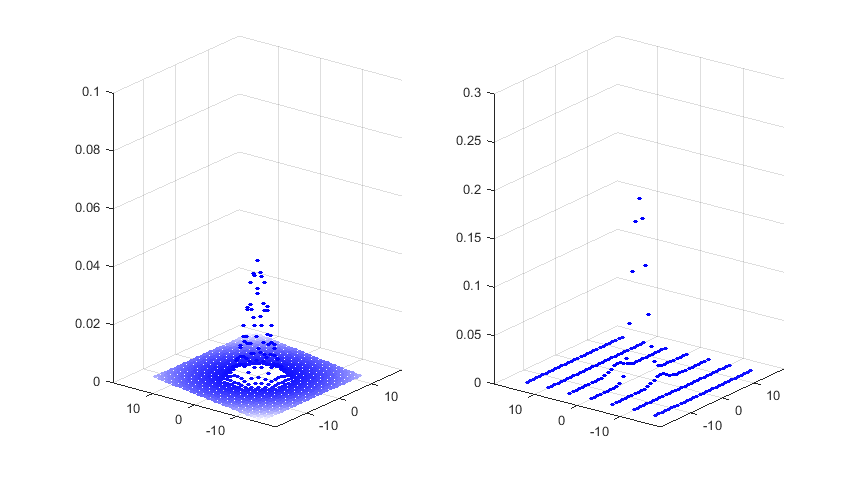
\includegraphics[scale = .45]{./figures/fig1.png}
        \caption{Gaussians with the same width over a lattice and its dual. Here the width is \(r = 5\).}
        \label{fig:Gaussian over Lattice}
    \end{figure}

\subsection{Hard Problems}
    \begin{figure}[h]
        \label{Figure: Problem Tree}
        \[\xymatrix{
            \text{GapSVP}_{\zeta, \gamma} \ar[dr]^{\text{Peikert}}\ar[d]_{\zeta\geq 2^{n/2}}&&\text{BDDP}\ar[dl]\\
            \text{GapSVP}_\gamma\ar[r]^{Q}\ar[u] &  \text{LWE}\ar[r]\ar[ur]^{???} & \text{SIS}\ar@<1ex>[l]^{\text{Q}}\\
                                &  \text{SIVP}\gamma\ar[u]^{\text{Q}}& \\
                                &  \text{SVP}_\gamma\ar[u]\ar[r]^{???} & \text{SG-PIP}\ar[l]
        }\]
        \caption{Problem Tree. The arrows indicate directions of reduction. E.g. solving SVP boils down to solving SIS. Quantum reductions are indicated with a Q. [Do not put arrows without arguing or referencing]}
    \end{figure}
    On Figure \ref{Figure: Problem Tree} we present many relations between lattice problems. In this thesis we mainly concern ourselves with the bottom part, mainly SVP\(_\gamma\). However, any attack further up in the tree would result in an attack on SVP. Therefore, the security of LWE and SIS is paramount to the security of any lattice based cryptosystem. \par
    
    Lets have a word about Ajtai. In his seminal paper\cite{Ajtai} he defined many of the hard problems that are used in lattice-based cryptography. More importantly, he showed that for many of these problems, there is a reduction from average-case to worst-case. This means that many problems related to lattices is as hard in the average case as they are in the worst case. This is an important aspect of cryptography, because if a problems only sometimes is hard, then the system is not secure. Having a reduction means that every instance of the given problem is as hard as an instance created to be as difficult to break as possible.\par
    
    A quantity which we are often interested in is the shortest vector in a given lattice. We define \(\lambda_1(\Lambda)\) (abbreviated \(\lambda_1\) when the context is clear) to be the this shortest vector. This definition can be extended to include more than one vector.
    \begin{definition}[Successive Minima]
        For a lattice \(\Lambda\), we define the \emph{\(i\)-th successive minima}
        \begin{align*}
            \lambda_i = \emph{min}\{r\suchthat\Lambda\emph{ contains } i \emph{ linearly independent vectors each of length }\leq r\}
        \end{align*}
    \end{definition}
    It is easy to see that \(0 < \lambda_1 \leq \lambda_2 \leq\dots\leq\lambda_n\). How hard these problems are depends in a large extent to which basis describes the lattice. Consider for instance a lattice \(\Lambda\) with an orthogonal basis. It is not hard \change{is it not hard?} to see that the shortest vector in such a lattice would be one of the basis vectors. We therefore have an attack in time \(O(n)\) to solve SVP. By changing the basis for a lattice to be orthogonal, or as orthogonal as possible, we might give ourselves an easier time solving SVP. However, there is no known polynomial algorithm that solves neither SIVP or SVP. By relaxing these problems to not find \emph{the} shortest vectors but only approximations, we give ourselves some room to maneuver.
    
    \begin{definition}[SVP\(_\gamma\)]
        Given a basis \(\mathcal{B}\) for a lattice \(\Lambda\), output the shortest vector \(\lambda_1\) up to a scaling factor \(\gamma\), I.e., output a non-zero vector with length \emph{at most} \(\gamma\lambda_1\).
    \end{definition}
    By choosing \(\gamma\) as large as we need to, this problem becomes trivial. Naturally, we want \(\gamma\) to be as small as possible. Current algorithms tend to have \(\gamma=\mathcal{O}(2^n)\)\needtodo{is this a proven upper limit?}, which looks like a bad approximation for something that should be short. In the way we extended the SVP to SIVP by requiring more short, linearly independent vectors, we extend the SVP\(_\gamma\) similarly:
    \begin{definition}[SIVP\(_\gamma\)]
        Given a basis \(\mathcal{B}\) of a lattice \(\lambda\), the problem SIVP\(_\gamma\) is to find \(n\) linearly independent vectors \emph{all } of length at most \(\gamma\lambda_n\)
    \end{definition}
    For this relaxed SVP-version we do have a polynomial time attack for sufficiently large approximation factor. We can use the revered LLL algorithm to recover a \(\gamma\)-approximate shortest vector in time \(O(n^6(\log B)^3\) where \(n\) is the lattice dimension, \(B\) is a bound for the euclidian length of the basis vectors and \(\gamma = O(2^n)\) \cite{Galteland}\improvement{find original source}.\par
    
    Decrypting \improvement{only talk theory?} ciphertexts in lattice based cryptography often means to find the closest vector to the given ciphertext. We therefore define the problem that describes this, again with the familiar scaling factor.
    \begin{definition}[CVP\(_\gamma\)]
    Given a basis \(\mathcal{B}\) of a lattice \(\Lambda\) and a vector \(y\in\RR\), the problem is the find a non-zero vector \(x\) such that \(||y-x||_2\leq\gamma \emph{dist}(\Lambda , y)\).
    \end{definition}
    It is intuitive that CVP and SVP should be related. We could try to use CVP to find the closest vector to 0 in the lattice, which would be the shortest vector as \(x - 0 = x\). This does not quite work as 0 is also a lattice point, and 0 will always be closest to 0 so this algorithms might output 0. We can do the reduction SVP\(\leq\)CVP as shown in Figure \ref{Fig: SVP to CVP Reduction}. 
    
    \begin{figure}
    \label{Fig: SVP to CVP Reduction}
    \begin{algorithm}[H]
    \DontPrintSemicolon
     SVP($\mathcal{B}$)\;
     \For{$i = 1 $ \KwTo $n$}{
      \(\mathcal{B}^i \leftarrow \left\{b_1,\dots ,2b_i,\dots , b_n\right\}\)\;
      \(x_i\leftarrow \) CVP(\(\mathcal{B}^i, b_i)\)\;
     }
      \Return min\(\left\{x_i - b_i\right\}\)
     
     \caption{SVP to CVP reduction.}
    \end{algorithm}
    \end{figure}
    For each iteration, the algorithms makes a new basis where element \(i\) is scaled by a factor \(2\). Then, we query a CVP oracle with this new basis and the un-scaled basis element. Without scaling, CVP would trivially return \(b_i\) in each case.\needtodo{Finish this proof}. This reduction can easily\improvement{easily?} be extended to the corresponding \(\gamma\)-approximated problems.\par
    \begin{definition}[Bounded Distance Decoding Problem]
    Let \(\mathcal{B}\) be a basis for the lattice \(\Lambda\). Given a point \(t\in\emph{span}(\mathcal{B})\) with the guarantee that \(\emph{min}_{v\in\Lambda}||v-t||\leq r\) for some known \(r\leq\lambda_1/2\), output the unique \(v\in\Lambda\) closest to \(t\).
    \end{definition}
    The BDDP problem is closely related to CVP, the only difference is that we are guaranteed that the target point is sufficiently close to a lattaice point.\needtodo{Check that this is the correct definition!}.
    
    \begin{definition}[Shortst Integer Solution (SIS)]
    Given \(\vec{a}_i\in\ZZ_q^n\), find small and non-trivial \(z_i \in\ZZ \) such that
    \begin{equation}
        \label{Eq: SIS}
        z_1\vec{a}_1 + z_2\vec{a}_2 + \dots + z_n\vec{a}_n = 0\;\;\in\ZZ_q^n
    \end{equation}
    In other words, \(\vec{z}A = 0\text{ mod } q\).
    \end{definition}
    Looking long and hard at the set 
    \begin{align*}
        \Lambda_q(A)^{\perp} := \left\{\vec{x}\in\ZZ\;|\; \vec{x}A = 0\quad\text{ mod }q\right\}
    \end{align*}
    which is the set of all solution of Equation \eqref{Eq: SIS}. It is not hard to see that this set is a lattice, and therefore solving SIS is equivalent  to finding a vector with small coefficients in the lattice \(\Lambda(A)^{\perp}\). It is important to note that this does \emph{not} mean that we find a short vector in the lattice, as a short vector can have very large coordinates. Ajtai\cite{Ajtai} showed that many lattice problems \change{Which ones?} are at least as hard as SIS (See Figure \ref{Figure: Problem Tree}. \par
    Another problem which is seemingly not related to lattices is called \emph{learning with errors}. The setup is a set of linear equations with some error.
    \begin{equation}
    \label{Equation: LWE}
        \begin{split}
            b_1 = & \;\langle \vec{s}, \vec{a}_1\rangle + e_1\\
            b_2 = & \;\langle \vec{s}, \vec{a}_2\rangle + e_2\\
            \vdots & \\
            b_k = & \;\langle \vec{s}, \vec{a}_k\rangle + e_k
        \end{split}
    \end{equation}
    where \(\vec{a}_i\leftarrow\ZZ_q^n\), the \(e_i\)-s are sampled from some distribution \(\chi\) and \(\vec{s}\in\ZZ_q^n\). The 'learning' part of the problem is to recover \(s\). Notice that without the error terms \(e_i\), this can be solved by Gaussian elimination if we have enough equations because \(\vec{A}\) will be invertible given enough equation\improvement{cite}. It is therefore natural to let \(k > n\) to have this problem make any sense. For clean notation we define a LWE-sample
    \begin{definition}
        Pick \(\vec{s}\leftarrow\ZZ_q^n\) and \(e\leftarrow\chi\). An \emph{LWE-sample} is a sample of the form \((a, b)\) where \(\vec{a}\leftarrow\ZZ_q^n\) and \( b = \langle \vec{s}, \vec{a}\rangle + e\). We say that an LWE-sample is a sample from the distribution \(A_{\vec{s}, \chi}\).
    \end{definition}
    Related to LWE are two problems; recovering\footnote[2]{Which acts like the secret key in cryptosystem based on LWE} \(\vec{s}\) and deciding whether the \(b_i\)-s are distributed according to the above selection \improvement{clearer language here} or if they are distributed uniformly.
    \begin{definition}[Search LWE]
        Given access to many LWE-samples, recover \(\vec{s}\).
    \end{definition}
    
    \begin{definition}[Decision LWE]
       Given access to many LWE-samples and \(A = (\vec{a}_1, \vec{a}_2,\dots ,\vec{a}_k)\), distinguish \((\vec{A}, \vec{b} = \vec{s}\vec{A} + \vec{e})\) from \((\vec{A}, \vec{u})\) where \(\vec{u}\) is distributed uniformly.
    \end{definition}
    
    A fact about decision-LWE and search-LWE is that they are equivalent. 
    \begin{proposition}
    search-LWE = decision-LWE
    \end{proposition}
    \begin{proof}
        \underline{search-LWE\(\leq\)decision-LWE}: This is trivial because if we can recover \(s\), then we can calculate \(\vec{e} = \vec{b} - A\vec{s}\) and check if \(\vec{e}\) is uniformly distributed. This is assuming that \(\vec{e}\) is \emph{not} uniformly distributed from the start, making decision-LWE impossible.\par
        \noindent\underline{decision-LWE\(\leq\)search-LWE}: Let \(\vec{s} = (s_1,\dots ,s_{k})\). We are going to find one coordinate of \(\vec{s}\) at a time. Pick a random \(r\leftarrow\ZZ_q\). We observe that 
        \[
            \begin{split}
                b_i' & =  \langle \vec{s}, \vec{a}_i  + (r, 0,\dots , 0)\rangle + e \\
                & = \langle \vec{s}, \vec{a}_i\rangle + s_1r + e
            \end{split}
        \]
        Now, since \(r\) was chosen uniformly at random, \(b_i'\) will also be uniformly distributed, unless \(s_1 = 0\). Therefore, we query the decision-LWE oracle on \(\big(\vec{b}^{'}, (\vec{s} + (r,0,\dots ,0))A + e\big)\). If decision-LWE decides that it is \emph{not} uniformly distributed we conclude that \(s_0 = 0\). Otherwise, we shift \improvement{Ague for shifting} \(\vec{s}\) by \(\vec{t} = (1,0, \dots, 0)\) and do that same thing with \(\vec{s} + \vec{t}\). Doing this \(q\) times will result in deciding what \(s_0\) is. Doing this for all \(s_i\) recovers \(\vec{s}\).
    \end{proof}\improvement{Can make this proof more detailed.}
    This means that we can regard both problems as one, namely LWE. We also have average case hardness of LWE.
    \begin{proposition}
        LWE is as hard in the average case as it is in the worst case.
    \end{proposition}
    \begin{proof}
        Let \(\mathcal{A}_{\vec{s}}\) denote a LWE-sample. Assume there is some set \(S\subseteq\ZZ_q^n\) such that \(|S|/|\ZZ_q^n| = 1/\text{poly}(n)\), i.e. \(S\) is not too small, and that LWE-samples where \(\vec{s}'\leftarrow S\), decision-LWE is easy. That is, we have a distinguisher \(A\) which can distinguish samples from \(\mathcal{A}_{\vec{s}'}\) from uniform ones. It is easy to see that the sample \(\{\vec{a}_i, \vec{b}_i + \langle \vec{a}_i, \vec{t}\rangle /q\}\) are samples from \(\mathcal{A}_{\vec{s}+\vec{t}}\). Therefore, given \emph{any} \(s\leftarrow\ZZ_q^n\), pick a uniformly random \(\vec{t}\leftarrow\ZZ_q^n\), and query \(A\) on 
        \begin{align*}
            \{\vec{a}_i, \vec{b}_i + \langle \vec{a}_i, \vec{t}\rangle/q\}.
        \end{align*}
        Since \(S\) is sufficiently large, we will, with high probability, eventually \(\vec{s} + \vec{t}\in S\) and we can solve the problem by querying \(A\). This means that if there exists a sufficiently large set \(S\) where decision-LWE is easy, then decision-LWE is easy \emph{for all} of \(\ZZ_q^n\). We conclude that no such set can exist \improvement{why can it not?}. Since decision-LWE \(=\) search-LWE we get that LWE is average case hard\change{Be more precise}.
    \end{proof}
    To illustrate the relationship between LWE and lattices, consider
    \begin{align*}
        \Lambda_q(A) = \left\{\vec{z}\suchthat\vec{z} = \vec{s}A\text{ mod } q \text{ for some }\vec{s}\in\ZZ_q^m\right\}.
    \end{align*}
    Given a point \(\vec{s}\vec{A}\) in the lattice \(\vec{y} = \vec{s}A + \vec{e}\) we can use CVP to recover \(\vec{s}A\) and solve \(\vec{b} = \vec{s}A\). If we also can guarantee that \(\vec{e}\) is 'short', the problem becomes BDDP.\par
    
    We now give an example of an attack on LWE. Given a LWE-sample \((\vec{a}, b = \langle \vec{s}, \vec{a}\rangle + e)\) and a divisor \(q'|q\), we can reduce the sample modulo \(q'\) to obtain
    \begin{align*}
        (\vec{a}' = \vec{a}\text{ mod } q', b' = \langle \vec{s}', \vec{a}' + e)
    \end{align*}
    where \(s' = s \text{ mod } q'\). Notice that the errors are still from the same distribution \(\chi\)\improvement{argue for this}. If we let \(q' = 1\) then \(\langle \vec{s}', \vec{a}'\rangle = 0\) so \(b = e\modulo\ZZ\). We not have two potential attacks. Firstly, if we can conclude that samples from \(\chi\) are not uniform modulo \(\ZZ\), then we have a distinguishing attack. We simply need to check whether \(b\in\RR/\ZZ\) are non-uniform.\par
    
    Secondly, we have a potential search attack. Assume that the errors from \(\chi\) usually does not wrap around modulo \(\ZZ\), that is the probability that an error is outside the interval \([-1/2, 1/2)\) is small. Symbolically,
    \begin{align*}
        \text{Pr}\left[e\not\in\left[-\frac{1}{2}, \frac{1}{2}\right)\right] \leq \varepsilon
    \end{align*}
    for a small \(\varepsilon\). We now have an attack: Let \(\Hat{e}\) be an error that does not wrap around. By definition of \(\hat{e}\), \(b - \hat{e} = \langle \vec{s}, \vec{a}\rangle\) so if we can collect enough such errors we can recover error-less LWE samples and solve LWE trivially by, for instance, Gaussian elimination. Since the probability that an error does \emph{not} wrap around is small, we can find enough such errors in short time.\par
    
    These two attack also work for other divisors of \(q\), but for simplicity we only describe it for \(q' = 1\).\improvement{why do we know these divisors?}. From these two attack we get two requirements for the error distribution \(\chi\): It must be statistically indistinguishable from uniform modulo \(\ZZ\), and the sufficiently many errors must wrap around modulo \(\ZZ\).\par
    
    If we not let \(\chi = D_r\) be a Gaussian of width \(r\) exceeding the smoothing parameter \(r \geq \eta_\varepsilon(\ZZ)\). We can for instance let \(r > \sqrt{n} \geq \eta_{2^{-n}}(\ZZ)\) as described in the worst-case hardness theorems from LWE\needtodo{find these sources, ez}. These errors wrap around modulo \(\ZZ\) with high probability \improvement{cite} and moreover \(b\modulo\ZZ\) are statistically close to uniform by the choice of the width of \(D_r\). 
    
\subsection{Ring-LWE}
    Before we discuss Ring-LWE we want to have a low-level discussion of a vector space. We define \(K_\RR := K\otimes\RR\). By fixing a \(\QQ\)-basis for \(K\), \(\{u_1, \dots , u_n\}\) such that we can write any \(\alpha\in K\) as \(\alpha = q_1u_1 + \dots + q_n u_n\). Now any element \(e\in K_\RR\) is of the form
    \begin{align*}
        e = (q_1, q_2, \dots , q_n)\otimes x = (q_1x,q_2x,\dots ,q_nx)
    \end{align*}
    for \(q_i\in\QQ\) and \(x\in\RR\). Since \(q_i x\in\RR\), we get that \(K_\RR\) is a vector space over \(\RR\) and hence isomorphic to \(\RR^n\). The vector space \(K_\RR\) is where the errors are drawn in the ring variant of LWE.\par
    
    For applications, \(\vec{s}\) is the secret key in cryptosystems based on LWE. Now, to have any chance of recovering \(\vec{s}\) we need to have more than \(n\) equations, so \(m = O(n)\) at least. The key size is therefore \(O(n^2)\) which is pretty big. As introduced in \cite{First R-LWE}, it is desirable to, instead of sampling from \(\ZZ_q^n\), sample from a certain ring. 
    \begin{definition}[Ring-LWE (R-LWE)]
        Let \(\OO_q = \OO/\langle q\rangle\). Pick a secret \(s\in \OO_q^\vee\). Let \(\chi\) be a distribution over \(K_{\RR}\). Sample \(a \leftarrow \OO_q\) uniformly and \(b\leftarrow (a\cdot b) + e \emph{ mod } qR^\vee\). A R-LWE sample is \((a, b)\). As before, the \emph{search} version is the recover \(s\) and the \emph{decision} version is to distinguish a R-LWE sample \((a, b)\) from one where \(b\) is sampled uniformly.
    \end{definition}
    Notice that the secret key is an element from the dual lattice \(\OO^\vee\). This will be discussed later. However, a definition where the samples are all taken from the non-dual \(\OO\) is equivalent to this definition, up to the error distribution \(\chi\)\cite{How Not To RLWE}. There is some 'tweaking' needed for this equivalence\needtodo{cite}. From Proposition \ref{Prop: Cancel Ideal} we have that\needtodo{convince yourself that this is the consequence of this prop!} there exists an bijection
    \begin{align*}
        \theta_t : \OO_q^\vee\rightarrow \OO_q,
    \end{align*}
    which we can extend to a map
    \begin{align*}
        \kappa_t:K_\RR/q\OO^\vee\rightarrow K_\RR/q\OO
    \end{align*}
    naturally. We use \(\kappa_t\) to transform a R-LWE sample \((a_i, b_i = s\cdot a_i + e_i)\) by
    \begin{align*}
        b_i' = \kappa_t(b_i) = t\cdot b_i = s'\cdot a_i + e_i'
    \end{align*}
    and keeping \(a_i\) fixed. \improvement{is it fixed or is the map on \(a_i\) fixed?} Notice that \(\kappa_t(s) = \theta_t(s)\), and since \(\theta_t\) is a bijection, we get that \(s'\) is distributed uniformly (since \(s\) was). This is therefore a valid R-LWE sample with error distribution \(t\cdot\chi\). Because \(\theta_t\) is a bijection, finding \(s'\) immidiately yields \(s\), so solving search for the transformed sample (with errors from \(t\cdot\chi\)) is equivalent to solving search for the original samples. Additionally, because \(\kappa_t\) sends uniform samples to uniform samples \needtodo{check} we get that the decision versions are equivalent as well.\par
    
    The cruical thing to note now is that we have a \emph{new} error distribution \(t\cdot\chi\). So if \(\chi\) itself satisfies the hardness properties of R-LWE, \(t\cdot\chi\) might not. The important part for hardness is the length of the errors. Consider therefore \(e\leftarrow\chi\). Under \(\kappa_t\) this becomes \(t\cdot e\) and has norm
    \begin{equation*}
        \begin{split}
            ||te|| = ||\sigma(te)|| & = ||(\sigma_1(te),\dots ,\sigma_n(te)||\\
                                    & = ||(\sigma_1(t)\sigma_1(e), \dots ,\sigma_n(t)\sigma_n(e)|| 
        \end{split}
    \end{equation*}
    In the trivial case where \(t\in\ZZ\) we get that \(t\cdot\chi\) is just a scaled version of \(\chi\), meaning a spherical distribution remains spherical. In general, however, \(t\in\OO^\vee\). Now if \(\chi\) is spherical, \(t\cdot\chi\) need not be since each \(i\)-th coordinate is scaled by \(\sigma_i(t)\). If the reductions rely on the \emph{largest} width of the Gaussians, we might try to scale each coordinate by the largest \(\sigma_i(t)\) such that we get a spherical distribution. However, this means that we need to change other parameters of the system to guarantee security. This is why keys from \(\OO_q^\vee\) makes for the tightest bounds and is the 'right' choice of ring.\par
    
    It is not obvious that R-LWE has the same hardness-properties as LWE, in particular a reduction from worst-case to average-case. However, R-LWE is connected to LWE in the following sense. If we let \(\mathcal{B}\) be a basis for \(R\), then for any \(a\in R_q\), we get that multiplication by \(a\) is represented by a matrix relative to the basis, say \(\vec{A}_a\). So given any \(s\in R_q\), we can represent it with respect to \(\mathcal{B}\) as \(\vec{s}\in \ZZ_q^n\). Now, given a R-LWE sample \((a, b = s\cdot a + e)\) we get \(n\) LWE samples
    \begin{align*}
        (\vec{A}_a, \vec{b} = \vec{s}\vec{A}_a + \vec{e}).
    \end{align*}
    It is not obvious now what the distribution of the columns of \(\vec{A}_a\) are uniformly distributed or that \(\vec{e}\) are. One attack on R-LWE makes sure that for any sample, we transform it into an \emph{error-less} LWE-sample. If we can generate enough of these, we can recover \(\vec{s}\) by linear algebra. \change{Move and make cohesive}\par
    
    Now, depending on how well we can represent the elements of \(R\), this version of LWE reduces the key-size by a factor of \(n\)\cite{First R-LWE}. However, we have introduced different structure on the sets we sample from. It is therefore not apparent that we have equally strong security on R-LWE as we do for 'regular' LWE. However, \cite{How Not To RLWE} shows that we can get as strong security on R-LWE as we did for LWE. In addition, under some assumptions we can get that search- and decision-R-LWE are equivalent.\par
    
    This relation between LWE and R-LWE is what is used in the security proof of certain instantiations of R-LWE. \par
    
    However, in \cite{First R-LWE} it was shown that we do indeed have similar properties. There is a \emph{quantum} reduction from worst-case SVP\(_\gamma\) on ideal lattices to the search variant of R-LWE. In addition, the R-LWE distributions are pseudorandom, meaning that the decision version of R-LWE is hard. These two properties are captured in the following theorem:
    \begin{theorem}[\cite{First R-LWE}]
        Suppose that it is hard for polynomial-time quantum algorithms to approximate the search version of the approximate SVP in the worst case on ideal lattices in \(\OO\) to within a fixed poly(n) factor. Then any poly(n) number of samples drawn from the distribution are pseudoreandom to any polynomial-time (possibly quantum) attacker.
    \end{theorem}
    
    We now describe two attacks, one one search and one on decision, of R-LWE from \cite{How Not To RLWE}. Both attacks are very similar to the attacks on 'regular' LWE. Let \(\frakq\) be an ideal divisor of \(\OO\). Given R-LWE samples
    \begin{align*}
        (a_i, b_i = s\cdot a_i + e_i)
    \end{align*}
    we transform them into samples modulo \(\frakq\) by setting \(a_i' = a_i \text{ mod } \frakq\) and \(b_i' = b_i \text{ mod } \frakq\). Now, \(b_i' = s'\cdot a_i' + e_i\) for \(s' = s\text{ mod } \frakq\). We have that reduction modulo \(\frakq\) maps uniform samples to uniform samples\needtodo{Argue for this?}. Now if \(\chi\text{ mod }\frakq\) is detectably non-uniform, we immediately have a distinguishing attack. For each candidate \(\hat{s}\in \OO/\frakq\) for \(s'\) check whether \(b_i' - \hat{s}\cdot a_i'\) are non-uniform. If such an \(\hat{s}\) exists, conclude that the distribution on the original \(b_i\) is \emph{not} uniform.\par
    
    If \(\chi\) has one or more coordinates that does not 'wrap around' modulo \(\ZZ\), then we can attack search by reducing the R-LWE samples to error-less LWE samples. If we can do this enough times we can solve LWE by, e.g., Gaussian elimination. \par
    
    We described an attack on LWE above, by reducing the samples modulo a divisor of \(q\). We can extend this attack to R-LWE by using a similar approach. Given an ideal divisor \(\frakq\) of \(q\OO\) we reduce the R-LWE samples to
    \begin{align*}
        (a_i'\modulo \frakq , b_i' = b_i\modulo \frakq).
    \end{align*}
    We have that \(a_i'\in\OO/\frakq\) and \(b_i' \in \RR^n/\frakq\OO ^\vee\). For each of the \(N(\frakq)\) candidates of the reduced secret \(s'\in\OO^\vee/\frakq\OO^\vee\), we check whether \(b_i' - a_i\cdot s'\in\RR^n/\frakq\OO^\vee\) are non-uniform. Like we assumed for simplicity that the divisor \(q'|q\) be \( q' = 1\), we now let \(\frakq = \OO\), such that we get maximum reduction:
    \begin{equation*}
        \begin{split}
            a' = & 0\modulo\OO^\vee\\
            b' = & e\modulo\OO^\vee
        \end{split}
    \end{equation*}
    Now, checking whether \(e\in K_{\RR}\) is non-uniform we have a distinguishing attack. If the error \(e\) does not 'wrap around', then we can reduce the samples to error-less LWE-samples and trivially recover the secret \(s\). 'Wrapping around' in this context means that the coefficients of the error vector \(\vec{e}\) corresponding to \(e\) via an appropriate basis does not wrap around. However, if we can guarantee that neither of these conditions are satisfied for a distribution \(\chi\), then none of these attacks work. Indeed, choosing a Gaussian with fitting width will be sufficient for both these conditions.\par
    
    We describe the reduction from the BDDP to R-LWE under certain conditions on the parameters. However, we show this reduction for a slightly different BDDP.
    \begin{definition}
        The \(q\)-BDDP\(_{\calI, d}\) is: given an instance \(y\) of BDD\(_{\calI, d}\) that has solution \(x\), find \(x\modulo q\calI\)
    \end{definition}
    Regev showed in \cite{Reg05} that there is a polynomial time reduction from BDDP\(_{\calI, d}\) to \(q\)-BDDP\(_{\calI, d}\). This means that we want to prove the second reduction in Figure \ref{fig:BDD to R-LWE Reduction}.
    \begin{figure}
        \[
        \xymatrix{\text{BDD}\ar[r] & q\text{-BDDP}\ar[r] & \text{R-LWE}}
        \]
        \caption{BDD to R-LWE reduction.}
        \label{fig:BDD to R-LWE Reduction}
    \end{figure}
    So, given a \(q\)-BDDP\(_{\calI^\vee, d}\) instance \(y = x + e\) with \(x\in\calI^\vee\) we want to make use of an R-LWE oracle \(\mathcal{L}\) and a DGS oracle \(\mathcal{D}_{\calI, r}\) to recover \(x\). Start by computing \(t\) such that \(t\cdot\calI\inverse\) is coprime to \(\langle q \rangle\). Now we use the R-LWE oracle \(\mathcal{L}\) as follows: \(\mathcal{L}\) will request samples untill it is confident that it has a solution. For each of these requets, sample \(z\leftarrow\mathcal{D}_{\calI, r}\) and compute the pair \((a, b)\) by
    \begin{equation*}
        \begin{split}
            a = &\theta_t\inverse (z\modulo q\calI) \\
            b = &(z\cdot y)/q + e'\modulo\OO^\vee.
        \end{split}
    \end{equation*}
    \needtodo{Talk about CRT, \(\theta(a)\) etc.}When we have helped \(\mathcal{L}\) enough times, it will output \(s\in\OO^\vee\). Finally compute \(\theta_t\inverse(s) \in \calI_q^\vee\). We now argue for correctness. To do this, prove that the \(a\) above is statistically close to uniform and the \(b\) is statistically close to a spherically bounded Gaussian.
    
\subsection{Why using \(\OO^\vee\) is Right}
    \begin{itemize}
        \item Emerges naturally from the BDD-to-LWE reduction from \cite{First R-LWE}.
        
        \item Good for cryptography: Allows for most errors while still decrypting correctly. Hardness theorems from \cite{First R-LWE} assume \emph{dual version} of R-LWE. Instantiating with 'correct' parameters but \emph{non-dual version} means that the tweak factor ruins the sperical error distribution.
        
        \item Natural for standard SIS-LWE 
    \end{itemize}
    


\subsection{Instantiating R-LWE}
     We can describe how to instantiate R-LWE in such a way that the attacks in \cite{How Not To RLWE} perform no better than known attacks (e.g. \cite{LWE Attack 1, LWE Attack 2}) against 'normal' LWE instantiated to have worst case hardness. This means that the width of the Gaussian is \(r>2\sqrt{n}\). We do this by relating parameters for R-LWE to LWE in such a way that we have sufficient parameters corresponding to the hardness-condition for worst-case hardness \emph{of LWE}. \par
     
     The following theorem is the only quantum step in some reductions regarding LWE and R-LWE:
     \begin{theorem}
        Let \(\alpha > 0\) and \(q\leq 2\) be an integer. There exists an efficient quantum algorithm that, given a fractional ideal \(\fraka\subseteq K\) and a number \(r\leq\sqrt{2}\cdot\eta_{\varepsilon}(\fraka)\) for some negligible \(\varepsilon = \varepsilon(n)\) such that \(r' := r\cdot\omega(\sqrt{\log n})/(\alpha q)\), an oracle to R-LWE\(_{q, \Psi_{\leq\alpha}}\), and a list of samples from the discrete Gaussian distribution \(D_{\fraka, r}\) outputs an independent sample from \(D_{\fraka, r'}\).
     \end{theorem}
     This theorem describes an iterative step for sampling from \(D_{r'}\) given enough samples from \(D_{r}\) where \(r' < r\). Additionally, we have a reduction from BDD to R-LWE for certain parameters. 

\newpage
\section{Find Generator}
The first part of solving SG-PIP is to find a generator for an ideal. We have a sub-exponential classical algorithm due to Biasse and Fieker\cite{Find Generator Classic} and a quantum polynomial time algorithm due to Biasse and Fang\cite{Find Generator Quantum}. As there exists a polynomial time algorithm to make such a generator short, having an efficient algorithm for finding the generator in the first place is the main problem of this attack. Both these results rely on the Generalized Rieman Hypothesis\improvement{Talk about this?}

\subsection{Some Notation}
The time complexity of algorithms here is often of a special form, so to have a cleaner notation we denote
\begin{align*}
    L_\Delta (a, c) = \text{e}^{c\log(|\Delta |)^a \log \log (|\Delta |)^{1 - a}},
\end{align*}
where \(\Delta\) is the discriminant of the field, clear by context. Many result also state that we find a \emph{compact representation}. 
\begin{definition}[Compact Representation]
    Let \(l > 0\) be a constant, a compact representation of \(\alpha\in\OO\) with respect to the integral basis \(\{\alpha_1, \dots ,\alpha_n\}\) of \(\OO\) is a set of exact representations of polynomial size algebraic numbers \(\gamma_j\) satisfying \(\alpha = \gamma_0\gamma_1^{l}\dots\gamma_k^{l^k}\), where \(k\) is polynomial in the size of the input. 
\end{definition}
The essence of this definition is that a compact representation is a way of representing an algebraic integer which is pretty short. For computational algebraic number theory, it would be bad to need too much memory to represent the values we are intereseted in. Lucklily, we have that for any \(\alpha\in\OO\), there exists a compact represenation\cite{Compact Representation}.\improvement{Do we need to talk more about this?}
\subsection{Classic Algorithm}
The main result of the classical part\cite{Find Generator Classic} is an algorithm that has time-complexity \(L(\frac{2}{3} + \varepsilon, c)\) for arbitrary \(\varepsilon > 0\) and \(c>0\). The algorithm is based on some heuristics. The method uses index calculus. Let \(\mathcal{B} = \{\frakp_1,\dots\frakp_N\}\) be a set of invertible prime ideals in \(\OO\) which generate \(\CL\). Consider the morphism\needtodo{show this is morphism?}
\[
    \xymatrix@R-2pc{
        \ZZ^N\ar[r]^{\varphi} & \mathcal{I}\ar[r]^{\pi} & \CL \\
        (e_1,\dots,e_N)\ar[r] &  \prod\limits_{i = 1}^N\frakp_i^{e_i}\ar[r] & \prod\limits_{i = 1}^N\left[\frakp_i \right]^{e_i}.
    }
\]
Now we have that \(\ZZ^N/\ker (\pi\circ\varphi )\simeq\CL\) so computing \(\CL\) comes down to computing \(\ker (\pi\circ\varphi)\). The kernel of this map is exactly the \((e_1,\dots ,e_N)\in\ZZ^N\) such that \(\frakp_1^{e_1}\dots\frakp_N^{e_N} = (\alpha) = \OO\). Using the index calculus method, we collect many relations of the form \(\prod_i\frakp_i^{{e_i^{(j)}}} = (\alpha_j)\) and put them in the rows of a relation matrix. If we can collect enough relations, the Smith Normal Form \needtodo{talk about SNF} will give us the structure of \(\CL\). Now picking \(X = (x_1,\dots,x_N)\) from the \emph{left} kernel of the relation matrix \(M\), we can make a unti \(\gamma_X = \alpha^{x_1}\dots\alpha_N^{x_N}\)\needtodo{Convince yourself}. We have that 
\begin{align*}
    (\gamma_X) = \frakp_1^{\sum_i x_ie_i^{(1)}}\dots\frakp_N^{\sum_i x_ie_i^{(N)}} = \frakp_1^0\dots\frakp_N^0 = (1) = \OO 
\end{align*}
and we get a way of finding units on \(\OO\). It is summarized in the following algorithm:
\begin{figure}
    \centering
    \begin{algorithm}[H]
     \DontPrintSemicolon
     Derive random relations in \(\CL _K\) between classes of elements of \(\mathcal{B}\)\;
     Let \(M\) be the matrix of relations for a generating system of the \(\ZZ\)-lattice of relations\;
     Compute \(\ker (M)\)\;
     Find a minimal generating set of the units of the form \(\gamma_X\) for \(X\in\ker (M)\)\;
     Find the group structure of \(\CL _K\) by the SNF of \(M\)\;
     Clarify the result.
     \caption{Finding a generator for a principal(?) ideal.}
    \end{algorithm}
\end{figure}
Theorems from \cite{Find Generator Quantum}
\begin{theorem}
    We have an algorithm to compute the ideal class group \(\CL _K\) and a compact representation of fundamental system of units of an order \(\OO\) of discriminant \(\Delta\) in a number field of degree \(n\) in time \(L_\Delta (a, c)\) where 
    \begin{itemize}
        \item \(a = 2/3 + \varepsilon\) for \(\varepsilon > 0\) arbitrarily small
        \item \(a = 1/2\) when \(n\leq \log (|\Delta|)^{3/4 + \varepsilon}\) for \(\varepsilon > 0\) arbitrarily small.
    \end{itemize}
\end{theorem}
This theorem is under GRH and some more heuristics. 

\subsection{Quantum Algorithm}
We present the main theorems of \cite{Find Generator Quantum}
\begin{theorem}
    There is a quantum algorithm for computing the \(S\)-unit group of a number field \(K\) in compact representation which runs in polynomial time in the parameters \(n=\emph{deg } K\), \(\log |\Delta |\), \(|S|\) and \(\emph{max}_{\frakp\in S}\{\log (N(\frakp )\}\). 
\end{theorem}

\begin{theorem}
    Under GRH, there is a quantum algorithm for computing the class group of the ring of integers \(\OO\) in a number field \(K\) which runs in polynimial time in the parameters \(n = \emph{deg } K\) and \(\log |\Delta |\).
\end{theorem}

\begin{theorem}
    There is a quantum algorithm for deciding if an ideal \(\fraka\in\OO\) is principal, and for computing \(\alpha\in\OO\) in compact representation such that \((\alpha) = \fraka\) which runs in polynomial time in the parameters \(n = \emph{deg } K\), \(\log N(\fraka)\) and \(\log |\Delta |\).
\end{theorem}


\newpage
\section{Recovering the Generator}
Given a generator of a principal ideal, the task is to make it as short as possible. As discussed \improvement{check that it actually is discussed}, if we can recover a short enough generator for the ideal, we are able to transform this generator to a short vector in the corresponding lattice. Creamer et.al. showed in \cite{Recover Short Gen} that there exists a polynomial algorithm to do this. We will present the main machinery for this algorithm and then present the details.

\begin{theorem}
\label{Thm: Recover Short Gen}
    Let \(D\) be a distribution over \(\QQ(\zeta)\) with the property that for any tuple of vectors \(\vec{v}_1,\dots ,\vec{v}_{\varphi(m)/2 - 1}\in\RR^{\varphi(m)/2}\) of Euclidian norm 1 that are orthogonal to the all-1 vector \(\vec{1}\), the probability that \(|\langle\emph{Log}(g), \vec{v}_i\rangle| < c\sqrt{m}\cdot (\log m)^{-3/2}\) holds for all \(i\) is at least \(\alpha\), where \(g\) is chosen from \(D\) and \(c\) is a universal constant. There there is an efficient algorithm that given \(g' = g\cdot u\), where \(g\) is chosen from \(D\) and \(u\in C\) is a cyclotomic unit, outputs an element of the form \(\pm\zeta^j g\) with probability at least \(\alpha\).
\end{theorem}
In addition to this theorem, we state a proposition that helps to solve a lattice problem. A very simple algorithm to solve BDDP is, on input basis \(\mathcal{B}\) and a target vector \(\vec{t}\), is called the round off algorithm and it simply outputs \(\mathcal{B}\cdot\lfloor({\mathcal{B}^\vee})^T\cdot\vec{t}\rceil\).
\begin{proposition}
\label{Prop: Round off Algorithm}
    Let \(\Lambda\) be a lattice over \(\RR\) with basis \(\mathcal{B}\), and let \(\vec{t} = \vec{v} + \vec{e} \in\RR^n\) for some \(\vec{v}\in\Lambda, \vec{e}\in\RR^n\). If \(\langle\vec{b}_j^\vee, \vec{e}\rangle\in\left[-\frac{1}{2},\frac{1}{2}\right)\) for all \(j\), then on input \(\vec{t}\) and basis \(\mathcal{B}\), the round-off algorithm outputs \(\vec{v}\).
\end{proposition}
\begin{proof}
Because \(\vec{v}\) is in the lattice have have that \(\vec{v} = \vec{z}\cdot\mathcal{B}\) for some integer vector \(\vec{z}\). Now, multiplying from the right on \(\vec{t} = \vec{v} + \vec{e}\) by \({(\mathcal{B}^\vee)^T}\) yields 
\begin{align*}
    \vec{t} {(\mathcal{B}^\vee)^T} = \vec{z} + \vec{e}\cdot{(\mathcal{B}^\vee)^T}
\end{align*} On the assumption on \(\langle\vec{b}_j^\vee, \vec{e}\rangle\) we get that
\begin{align*}
    \lfloor\vec{t} {(\mathcal{B}^\vee)^T}\rceil = \lfloor \vec{z} + \vec{e}\cdot{(\mathcal{B}^\vee)^T} \rceil = \vec{z}
\end{align*}
because \(\vec{z}\) is an integer vector.
\end{proof}
Now, looking hard at Theorem \ref{Thm: Recover Short Gen}, there are two main aspects of this result. There is a lattice, called the \emph{log-unit lattice} which will be defined later, that is related to orthogonality of \(\vec{1}\). We see elements from this lattice in the inner product in Theorem \ref{Thm: Recover Short Gen}. In the same inner product, we recognize a bound for an inner product, which relates to the round-off algorithm, Proposition \ref{Prop: Round off Algorithm}. If we can achieve this bound with non-negligible probability (related to \(\alpha\)), then we can solve BBDP. In this chapter we discuss the various aspects of this method, as described in \cite{Recover Short Gen}.
\subsection{Some More Background}
We now regard a number field \(K = \mathbb{Q}[\zeta_m]\), which can be embedded into \(\mathbb{C}\). The embeddings \(\sigma_j:\omega\mapsto\omega^j\) come in conjugate pairs, I.e. \(\sigma_j = \compconj{\sigma{-j}}\). Since we are mainly concerned by magnitudes, we index the embeddings over the multiplicative quotient group \(G = \ZZ_m^\vee/\{\pm 1\}\). We can then define the logarithmic embedding
\begin{definition}
The \emph{logarithmic embedding} is defined as
\begin{equation*}
    \begin{split}
        \emph{Log}:&\; \QQ[\zeta_m]\rightarrow \RR^{\varphi(m)}\\
                   & a\mapsto (\log |\sigma_j(a)|)_{j\in G}
    \end{split}
\end{equation*}
so any element \(a\) is mapped to a vector in \(\RR^{\varphi(m)}\). \improvement{did we talk about geometry?} It can be shown, by the Dirichlet Unit Theorem \improvement{talk about this?} that the image of Log under \(\OO_K^\vee\) is a full rank lattice of the linear subspace of \(\RR^{\varpi(m)}\) orthogonal to \(\vec{1}\). We refer to this lattice as the \emph{log-unit lattice}.
\end{definition}
Moreover, we want some cyclotomic units my man
\begin{definition}[Cyclotomic Units]
Let \(A\) be the multiplicative group generated by 
\begin{align*}
    \left\{\pm\zeta_m, 1 - \zeta_m^s\suchthat 1<s\leq m - 1  \right\},
\end{align*}
then the group of \emph{cyclotomic units} is defined as
\begin{align*}
    C = A\cap\OO_{\QQ[\zeta_m]}.
\end{align*}
\end{definition}
The group of cyclotomic units is the units of \(\QQ[\zeta_m]\). These units are hard to determine for general number fields\cite{Intro To Cyclotomic Fields}. We also have a nice expression for the generators of \(C\).
\begin{proposition}
Let \(m\) be a prime power, and define \(b_j := z_j/z_1 = (\zeta^j - 1)/(\zeta - 1)\). The group of cyclotomic units \(C\) is generated by \(b_j,\;\;j\in G\backslash \{1\}\)
\end{proposition}
\begin{proof}
See \cite{Intro To Cyclotomic Fields} probably. \needtodo{fix}
\end{proof}
We can notice that Log \(C\) is a sublattice of Log \(\OO^\vee\). In the algorithm, we find elements in Log \(C\). This might seem like a problem, but it is conjectured that \(\OO^\vee = C\) in many cases. It is shown for many power of 2 \(m\)-s \improvement{reference}.\par
To use the theorem, we need a bound of the norm of the basis elements of Log \(C\). Since \(b_j\) generate \(C\), and noticing that Log \(b_j = \) Log \(b_{-j}\) \improvement{Argue for this}, we define
\begin{align*}
    \vec{b}_j = \text{Log }b_j\quad j\in G\backslash\{ 1\}
\end{align*}
These \(\vec{b}_j\) form a basis for Log \(C\). Now, if we can bound the norm of the dual-vectors \(\vec{b}_j^\vee\), we can use the round-off algorithm to solve the BDDP in this lattice. This is essentially \cite{Recover Short Gen}. The following result does just that.

\begin{proposition}
    Let \(m= p^k\) be a prime power \(p^k\) and let \(\{\vec{b}_j^\vee\}_{j\in G\backslash \{1\}}\) be the dual basis to \(\{\vec{b}_j\}_{j\in G\backslash \{1\}}\). Then all the norms of \(\vec{b}_j^\vee\) are equal and
    \begin{align*}
        ||\vec{b}_j^\vee||^2 \leq 2k|G|\inverse\cdot(l(m)^2+O(1)) = O(m\inverse\cdot\log ^3 m).
    \end{align*}
\end{proposition}
We need a bit more machinery to prove this proposition. Recall that 
\begin{align*}
    b_j = z_j/z_1.
\end{align*}
We therefore define
\begin{align*}
    \vec{z}_j := \text{Log }z_j = \vec{b}_j + \vec{z}_1
\end{align*}
so that, for instance, \(\vec{z}_2 = \text{Log }(\zeta^2 - 1)\). Next, set up a \(G\times G\)-matrix \(\Vec{Z}\) by letting the \(j\)-th column of \(\vec{Z}\) be \(\vec{z}_{j\inverse}\). It looks something like this:
\begin{align}
    \vec{Z} = \left(\begin{tabular}{cccc}
           \(\log |\zeta^{1\cdot 1\inverse}-1|\) & \(\log |\zeta^{1\cdot 2^{-1}}-1|\) & \(\dots\) & \(\log |\zeta^{1\cdot k\inverse}-1 |\)\\
           \(\log |\zeta^{2\cdot 1\inverse}-1|\) & \(\log |\zeta^{2\cdot 2^{-1}}-1|\) & \(\dots\) & \(\log |\zeta^{2\cdot k\inverse} -1|\)\\
           \(\vdots\) & \(\vdots\) & \(\ddots\) & \(\vdots\) \\
           \(\log |\zeta^{k\cdot 1\inverse}-1|\) & \(\log |\zeta^{k\cdot 2\inverse}-1|\) & \(\dots\) & \(\log |\zeta^{k\cdot k\inverse}-1|\)
        \end{tabular}\right).
\end{align}
We can notice that this is exactly the \(G\)-circulant matrix associated with \(\vec{z}_1\) \improvement{really?}. For each eigenvector of \(\chi\in\hat{G}\), let \(\lambda_\chi = \langle \vec{z}_1, \chi\rangle\) be the corresponding eigenvalue. We then have that
\begin{proposition}
    For all \(j\in G\backslash\{ 1 \}\) we have that 
    \begin{align*}
        ||\vec{b}_j^\vee|| = |G|\inverse\cdot\sum\limits_{\chi\in \hat{G}\backslash \{ 1 \}}|\lambda_\chi |^2
    \end{align*}
\end{proposition}
\begin{proof}
Hei
\end{proof}
Now we have a bound for the length if the lattice vectors of the log-unit lattice. We have now the theory needed to prove Theorem \ref{Thm: Recover Short Gen}.
\begin{proof}
We are given an element \(g' = g\cdot u\). Now, applying the logarithm on both sides yields
\begin{align*}
    \text{Log }g' = \text{Log }g + \text{Log }u.
\end{align*}
By the assumptions of the distribution \(D\), the output of the round-off algorithm is correct, I.e. \(\text{Log }u\in\text{Log }C\). Next, we find, by linear algebra, coefficients \(a_j\) such that 
\begin{align*}
    \text{Log }u = \sum a_j\vec{b}_j.
\end{align*}
Since \(\vec{b}_j\) form a basis this can be done efficiently. Next, compute
\begin{align*}
    u' = \prod b_j^{a_j}.
\end{align*}
Since the kernel of the logarithmic embedding is the roots of unity \(\zeta\), we get that \(\text{Log }u' = \text{Log }u\) and conclude that \(u' = \pm\zeta^j u\) for some sign and some \(j\). Therefore we have that \(g'/u' = \pm\zeta^j u\) for some, possibly different, sign and \(j\). This finishes the proof.
\end{proof}
If we can find some bounds on certain lattice-vectors, then we are pretty golden. We therefore define the \emph{covering radius} of the lattice.
\begin{definition}[Covering Radius]
    The \emph{covering radius}, with respect to the \(p\)-norm, of a lattice \(\Lambda\) is defined as
    \begin{align*}
        \mu^{(p)}(\Lambda) = \max_{\vec{v}\in\emph{span}\Lambda}\;\min_{\vec{x} - \vec{v}}||\vec{x} - \vec{v}||_p.
    \end{align*}
\end{definition}
Geometrically, this is the smallest radius required to cover the whole lattice with balls centered around each lattice point. Now we introduce some notation and variables to get some bounds. 
\begin{proposition}
    Let \(H\) be the subspace of \(\RR^{\varphi(m)/2}\) spanned by Log \(\OO^\vee\). For any \(g\in R\), let \(\mathcal{I} = g\OO\) be the ideal generated by \(g\). Denote \(\vec{g} = \text{Log }g\) and write it as \(\vec{g} = s\vec{1} + \vec{g}_H\) where \(\vec{g}_H\in H\)\improvement{show that his is possible}. Then there exists an efficient algorithm that, given any \(h_H\in g_H + \text{Log }C\), outputs a generator \(h\) of \(\mathcal{I}\) such that 
    \begin{align*}
        ||h|| \leq \sqrt{\varphi (m)}\exp(||\vec{h}_H||_\infty ) \cdot S(\mathcal{I})
    \end{align*}
    where \(S(\mathcal{I}) = N(\mathcal{I})^{1/\varphi(m)}\) is the dimension-normalized norm.
\end{proposition}
Note that we have the subspace \(H\subseteq \OO\), which is the space orthogonal to \(\vec{1}\). Therefore we can decompose any vector \(g\in\OO\) as an element in \(H\) plus an element in the space spanned by \(\vec{1}\). Hence, the decomposition \(\vec{g} = s\vec{1} + \vec{g}_H\) always exists. Now we proceed with the proof.\needtodo{Make sure this is correct argument.}
\begin{proof}
    We begin by computing \(\vec{u} := h_H - g_H\) which is an element in \(\text{Log} C\) by definition. Then compute \(a_j\in\ZZ\) such that \(\vec{u} = \sum a_j\vec{b}_j\) and output \(h = \prod b_j^{a_j}\). Now, since \(\vec{h} := \text{Log }h = \text{Log }g + \vec{u} = s\vec{1} + h_H\) we have that
    \begin{align*}
        ||h||^2 = \sum\limits_{i\in\ZZ^\vee_m}|\sigma_i (h)|^2 \leq \varphi(m)\cdot\exp(||\vec{h}||_\infty)^2 = \varphi(m)\exp (||h_H||_\infty)^2\cdot S(\mathcal{I}
        )^2
    \end{align*}
    where the first inequality follows by
    \begin{align*}
        \text{Arguemnt here}
    \end{align*}
    and the last equality follows because
    \begin{align*}
        N(\mathcal{I}) = N(g) = \prod\limits_{i\in\ZZ^\vee_m}\sigma_i (g) = \prod\limits_{i\in G}|\sigma_i(g)|^2 = \exp (2\langle\vec{g}, \vec{1}\rangle) = \exp (s\cdot\varphi (m)).
    \end{align*}
\end{proof}
\subsection{Discussion}
The main machinery of Theorem \ref{Thm: Recover Short Gen} relies on some constraints on a distribution. This is discussed in \cite{Recover Short Gen} where it is proven that many natural distributions satisfies the conditions of the theorem. However, a crypto scheme which uses a distribution which doesn not is not as vulnerable to this attack. However, one might not want such a distribution as this can possibly make the system slow or weak in other respects \needtodo{find claims to back this up}.\par
In addition, the algorithm described in Theorem \ref{Thm: Recover Short Gen} only works for inputs \(g' = g\cdot u\) for a cyclotomic unit \(u\), whereas we want the algorithm to work for general units in \(\OO^\vee\)\improvement{correct right?}. As discussed in \cite{Recover Short Gen} this should not be a problem. It is conjectures that the index of units over cyclotomic units is small, and there are well backed heuristics and computation that show this \needtodo{references}. If the index is small, we can enumerate over the cosets, which there are few of, and run the algorithm a number of times equal the index. This is the only heuristic in this algorithm.\par

\newpage
\section{SVP}
The field of lattice theory got a lot of attention when Ajtai\cite{Ajtai} showed a reduction from many worst case problems to average case problems\needtodo{right way of reduction?}. This made it a lot easier for provable security of cryptographic schemes based on lattices. \par
In addition, lattice have proven resistant to quantum computer attacks\improvement{Find source for this}. However, as we are going to show in this section, for some structured lattices and some problems, there exists quantum polynomial time algorithms.\needtodo{True?}\par
From the discussion of Section \(a \text{ and } b\), we get the following theorem.
\begin{theorem}
There is an efficient quantum algorithm for solving \(\text{SVP}_\gamma\) with approximation factor \(\gamma = O(\sqrt{m\log m})\).
\end{theorem}
\begin{proof}
Firstly, we apply a quantum algorithm to find a generator for the principal ideal we are interest in\improvement{talk about this}. We then use the methods described in this section to recover a short generator based on this.
\end{proof}

We have shown that there exists a quantum polynomial time algorithm to find a generator for the ideal \(\ZZ[X]/\langle f(x) \rangle\). We have also shown a polynomial time algorithm to make this generator short. This means that cryptosystems based on principal ideal lattices are not secure against quantum computers. Sometimes such cryptosystems use the generator as the public key, which means that these systems are not secure against classical computers either.  \improvement{Show which systems} We have not shown that ideal lattices are insecure in general. However, if the cryptosystems does not disallow principal ideal lattices, then the attacks discussed will be able to attack these systems if we, by chance, choose a principal ideal in the cryptographic system. However, it was shown/argued\change{change} in \cite{Identifying Ideal Lattices} that a randomly chosen lattice is practical never ideal. This means that this quantum attack on SVP will, in practice, never work unless we purposefully instantiate with basis for an ideal lattice.

\newpage
\begin{thebibliography}{99}
\bibitem{NTRU} Hoffstein, J., Pipher, J., Silverman, J.H.: \emph{NTRU: a ring-based public key cryptosystem}\needtodo{Publisher and Year}

\bibitem{Galteland} Herman Galteland, \emph{Fully Homomorphic Encryption Schemes}, 2015, Master Thesis, NTNU\needtodo{Year and published(?)}

\bibitem{Gentry} Gentry C., \textit{Fully Homomorphic Encryption Using Ideal Lattices}, Proceedings of the forty-first annual ACM symposium on Theory of computing p. 169-178, 2009

\bibitem{Short Sticleberg} Cramer R., Ducas L., Wesolowski B. (2017) Short Stickelberger Class Relations and Application to Ideal-SVP. In: Coron JS., Nielsen J. (eds) Advances in Cryptology – EUROCRYPT 2017. Lecture Notes in Computer Science, vol 10210. Springer-Verlag, Cham \improvement{Springer is Springer-Verlag?}

\bibitem{Recover Short Gen} Cramer R., Ducas L., Peikert C., Regev O. \emph{Recovering Short Generators of Principal Ideals in Cyclotomic Rings} Advances in Cryptography - EUROCRYPT 2016 II p. 550, Springer-Verlag

URL: \url{https://eprint.iacr.org/2015/313.pdf}

\bibitem{Recover2}
Espitau, T. et. al. \emph{Computing generator in cyclotomic integer rings}, EUROCRYPT 2016 I, Springer\needtodo{Make sure this is right source}

URL: \url{https://eprint.iacr.org/2016/957.pdf}

\bibitem{Reduction PG-PIP LWE} Peikert, C., \emph{Public-Key Cryptosystems from the
Worst-Case Shortest Vector Problem} [PUBLISHED BY?]

URL: \url{http://people.csail.mit.edu/cpeikert/pubs/svpcrypto.pdf}

\bibitem{Ajtai}  Ajtai, M., \emph{Generating hard instances of lattice problems} Quaderni di Matematica 2004

\url{URL: http://www.aracneeditrice.it/pdf/9788879994132.pdf}

\bibitem{Peikert Reduction} Peikert, C., \emph{Public-Key Cryptosystems from the Worst-Case Shortest Vector Problem}

\url{URL: https://web.eecs.umich.edu/~cpeikert/pubs/svpcrypto.pdf}

\bibitem{Intro To Cyclotomic Fields} Washington, L.C., \emph{Introduction to Cyclotomic Fields}, Graduate Texts in Mathematics,
vol. 83. Springer-Verlag, New York, 1st edition 1982

\bibitem{Prime Discriminant Division Theorem}
URL: \url{http://www.math.uconn.edu/~kconrad/blurbs/gradnumthy/disc.pdf}

\bibitem{Classic Recover}
URL: \url{https://arxiv.org/abs/1503.03107}

\bibitem{Lattice Beginner} Chi, D., et. al. \emph{Lattice Based Cryptography for Beginners}  URL: \url{https://eprint.iacr.org/2015/938.pdf}

\bibitem{Gjorsteen Lattice Intro} Gjørsteen, K., \emph{Lattice-Based Cryptography} \\URL \url{https://wiki.math.ntnu.no/_media/tma4160/lattice-i.pdf}:

\bibitem{Estimate Security} Rückert, M., Schneider, M., \emph{Estimating the Security of Lattice-based Cryptosystems} URL: \url{https://eprint.iacr.org/2010/137.pdf}

\bibitem{Basic Algebraic Number Theory} Oggier, F., \emph{Introduction to Algebraic Number Theory}, lecture notes given at NTU from January to April 2009 and 2010. URL \url{http://www1.spms.ntu.edu.sg/~frederique/ANT10.pdf}

\bibitem{Find Generator Classic} Biasse, J., Fieker, C. (2014). \emph{Subexponential class group and unit group computation in large degree number fields}. LMS Journal of Computation and Mathematics, 17(A), 385-403. URL: \url{https://www.cambridge.org/core/services/aop-cambridge-core/content/view/S1461157014000345}

\bibitem{Find Generator Quantum} Biasse, J.-F., Groves, M., \emph{A polynomial time quantum algorithm for computing class groups and solving the principal ideal problem in arbitrary degree number fields}\improvement{Different name some places}, In SODA 2016.

\bibitem{Compact Representation} Tiel, C., \emph{Short Proofs Using Compact Representations of Algebraic Integers}, Journal of Complexity p.310-329 Volume 11 Issue 3, 1995

\bibitem{Find Generator Quantum 2} Biasse, Song, \emph{On the quantum attacks against schemes relying on the hardness of finding a short generator of an ideal in \(\QQ(\zeta_{p^n})\)}, URL: \url{http://cacr.uwaterloo.ca/techreports/2015/cacr2015-12.pdf}

\bibitem{First R-LWE} Vadim Lyubashevsky, Christ Peikert, Oded Regev, \emph{On Ideal Lattices and Learning with Errors Over Rings}, EUROCRYPT 2010: 1-23

\bibitem{How Not To RLWE} Peikert C. (2016) How (Not) to Instantiate Ring-LWE. In: Zikas V., De Prisco R. (eds) Security and Cryptography for Networks. SCN 2016. Lecture Notes in Computer Science, vol 9841. Springer, Cham

\bibitem{Ideal Lattice Proof} Lyubashevsky, V., Miccianicio, D., \emph{Generalized compact knapsacks are collision resistant}, full version.\\
\url{https://pdfs.semanticscholar.org/a406/d27a16be28b858a36ba16ac7a72316177691.pdf}

\bibitem{Reg05} Regev, O., \emph{On Lattices, Learning with Errors, Random Linear Codes, and Cryptography}, STOC 2005 p. 84-93\\
URL: \url{https://dl.acm.org/citation.cfm?doid=1060590.1060603}

\bibitem{Smoothing Parameter Proof} Micciancio, D., Regev, O., \emph{Worst-case to average-case reductions based on Gaussian measures}\change{fix this reference}\\\url{https://cims.nyu.edu/~regev/papers/average.pdf}

\bibitem{Identifying Ideal Lattices} Ding, J., Lindner, R., \emph{Identifying Ideal Lattices}\change{find publisher} \\\url{https://eprint.iacr.org/2007/322.pdf}

%_________________ATTACKS ON LWE_________________%
\bibitem{LWE Attack 1} Arora, S., Ge, R.: \emph{New algorithms for learning in presence of errors}. In: In: Aceto, L., Henzinger, M., Sgall, J. (eds.) ICALP 2011, Part I. LNCS, vol. 6755, pp. 403-415. Springer, Heidenlberg (2011).\improvement{Stolen source, read?}

\bibitem{LWE Attack 2} Blum, A., Kalai, A., Wasserman, H.: \emph{Noise-tolerant learning, the parity problem, and the statistical query model}. J. ACM \textbf{50}(4), 506-519 (2003)

\bibitem{Bound on Size of Sample from Gaussian} Banaszczyk, W., \emph{New bounds in some transference theorems in the geometry of numbers}, Matematische Annalen, 296(4):625-635, 1993\improvement{have not read}

\bibitem{Error Tweak} Peikert. C., \emph{Lattice Cryptography for the Internet} \\
URL: \url{https://web.eecs.umich.edu/~cpeikert/pubs/suite.pdf}

\end{thebibliography}

\end{document}